\section*{Введение}

В данной лабораторной работе рассматриваются методы линейной фильтрации сигналов. Линейная фильтрация является важным инструментом обработки сигналов, основанным на использовании линейных дифференциальных уравнений и передаточных функций.

\textbf{Цель работы:} изучение методов линейной фильтрации, спектрального дифференцирования и их практического применения для обработки различных типов сигналов.

\textbf{Задачи:}
\begin{enumerate}
    \item Исследование спектрального дифференцирования
    \item Изучение линейных фильтров первого порядка
    \item Анализ специальных фильтров для устранения помех
    \item Применение линейной фильтрации к биржевым данным
\end{enumerate}

\section*{Задание 1. Спектральное дифференцирование}

\subsection*{Постановка задачи}

Рассматривается сигнал $y = \sin(t)$ с добавленным шумом. Требуется сравнить различные методы вычисления производной:
\begin{itemize}
    \item Численное дифференцирование по формуле $(y(k+1) - y(k))/dt$
    \item Спектральное дифференцирование через преобразование Фурье
    \item Истинная производная $\cos(t)$
\end{itemize}

\subsection*{Методология}

\textbf{Параметры эксперимента:}
\begin{itemize}
    \item Временной интервал: $t \in [-100, 100]$
    \item Шаг дискретизации: $dt = 0.1$
    \item Исходный сигнал: $y = \sin(t)$
    \item Шум: $a \cdot (\text{rand}(t) - 0.5)$, где $a = 0.1$
\end{itemize}

\textbf{Алгоритм спектрального дифференцирования:}
\begin{enumerate}
    \item Вычисление Фурье-образа сигнала с помощью численного интегрирования
    \item Умножение Фурье-образа на $i\omega$ для получения спектральной производной
    \item Обратное преобразование Фурье для восстановления производной во временной области
\end{enumerate}

\begin{figure}[H]
    \centering
    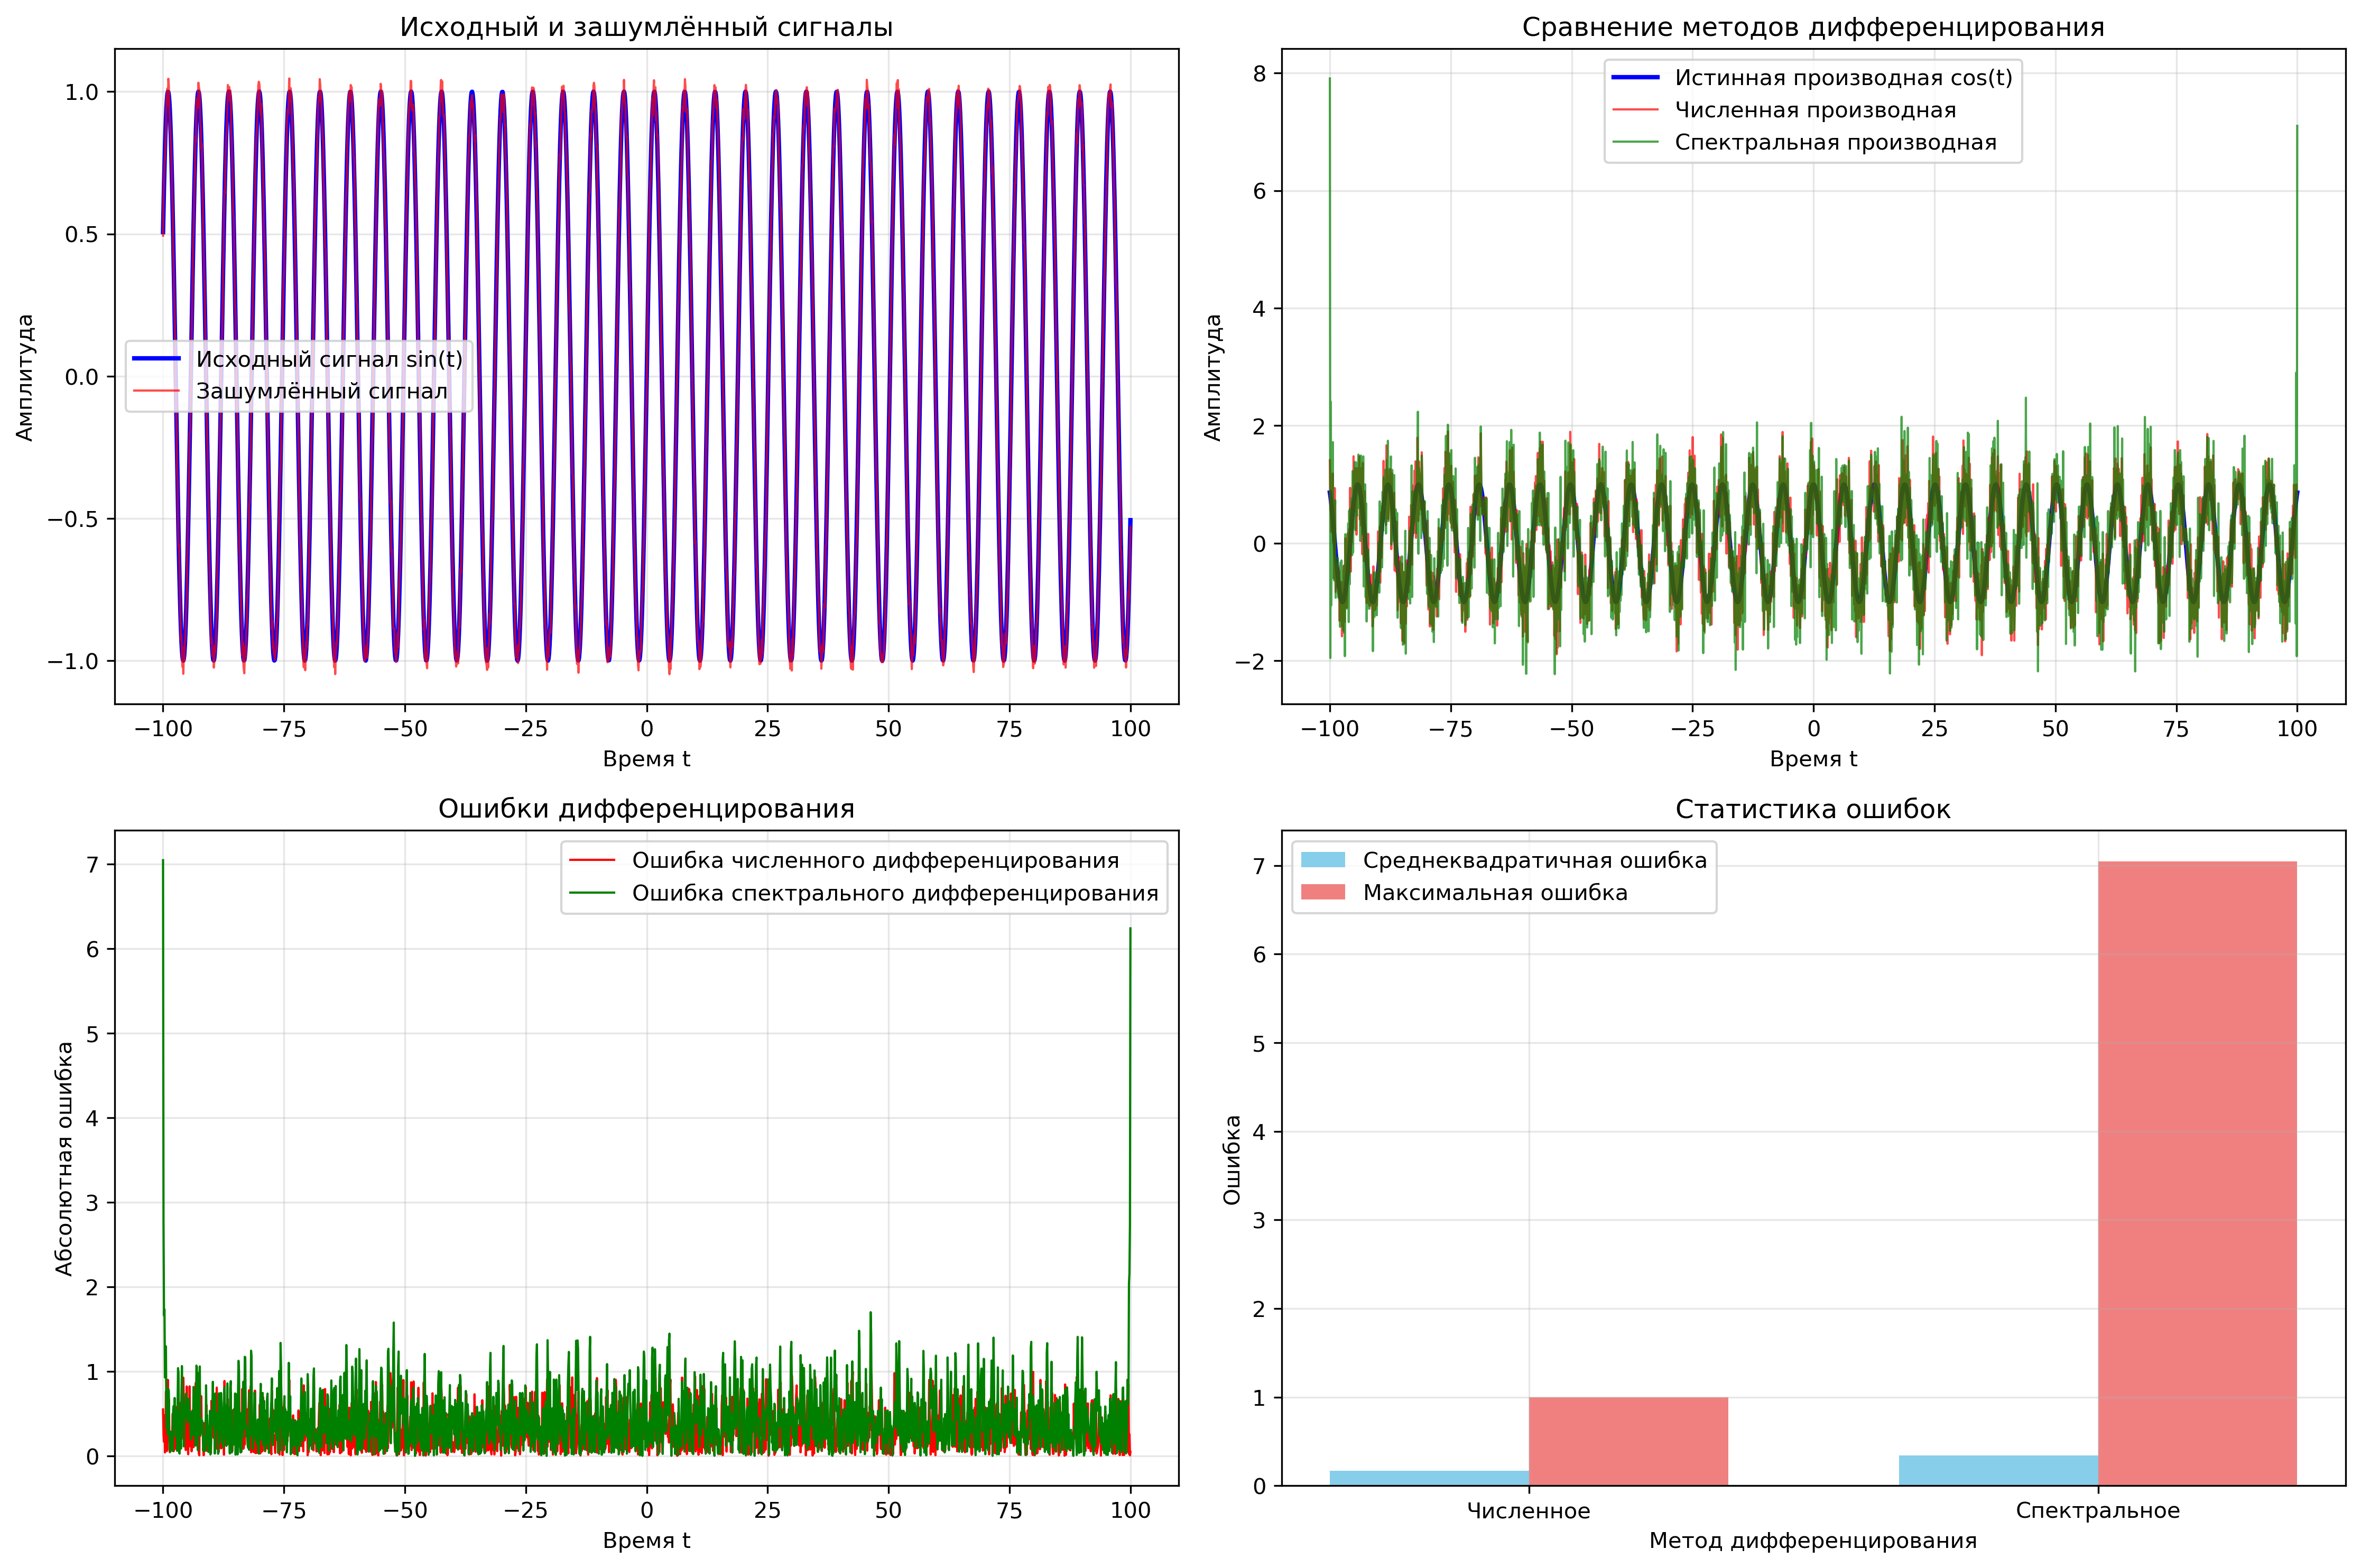
\includegraphics[width=0.8\textwidth]{images/task1/spectral_differentiation_comparison.png}
    \caption{Сравнение методов дифференцирования}
    \label{fig:spectral_diff_comparison}
\end{figure}

\begin{figure}[H]
    \centering
    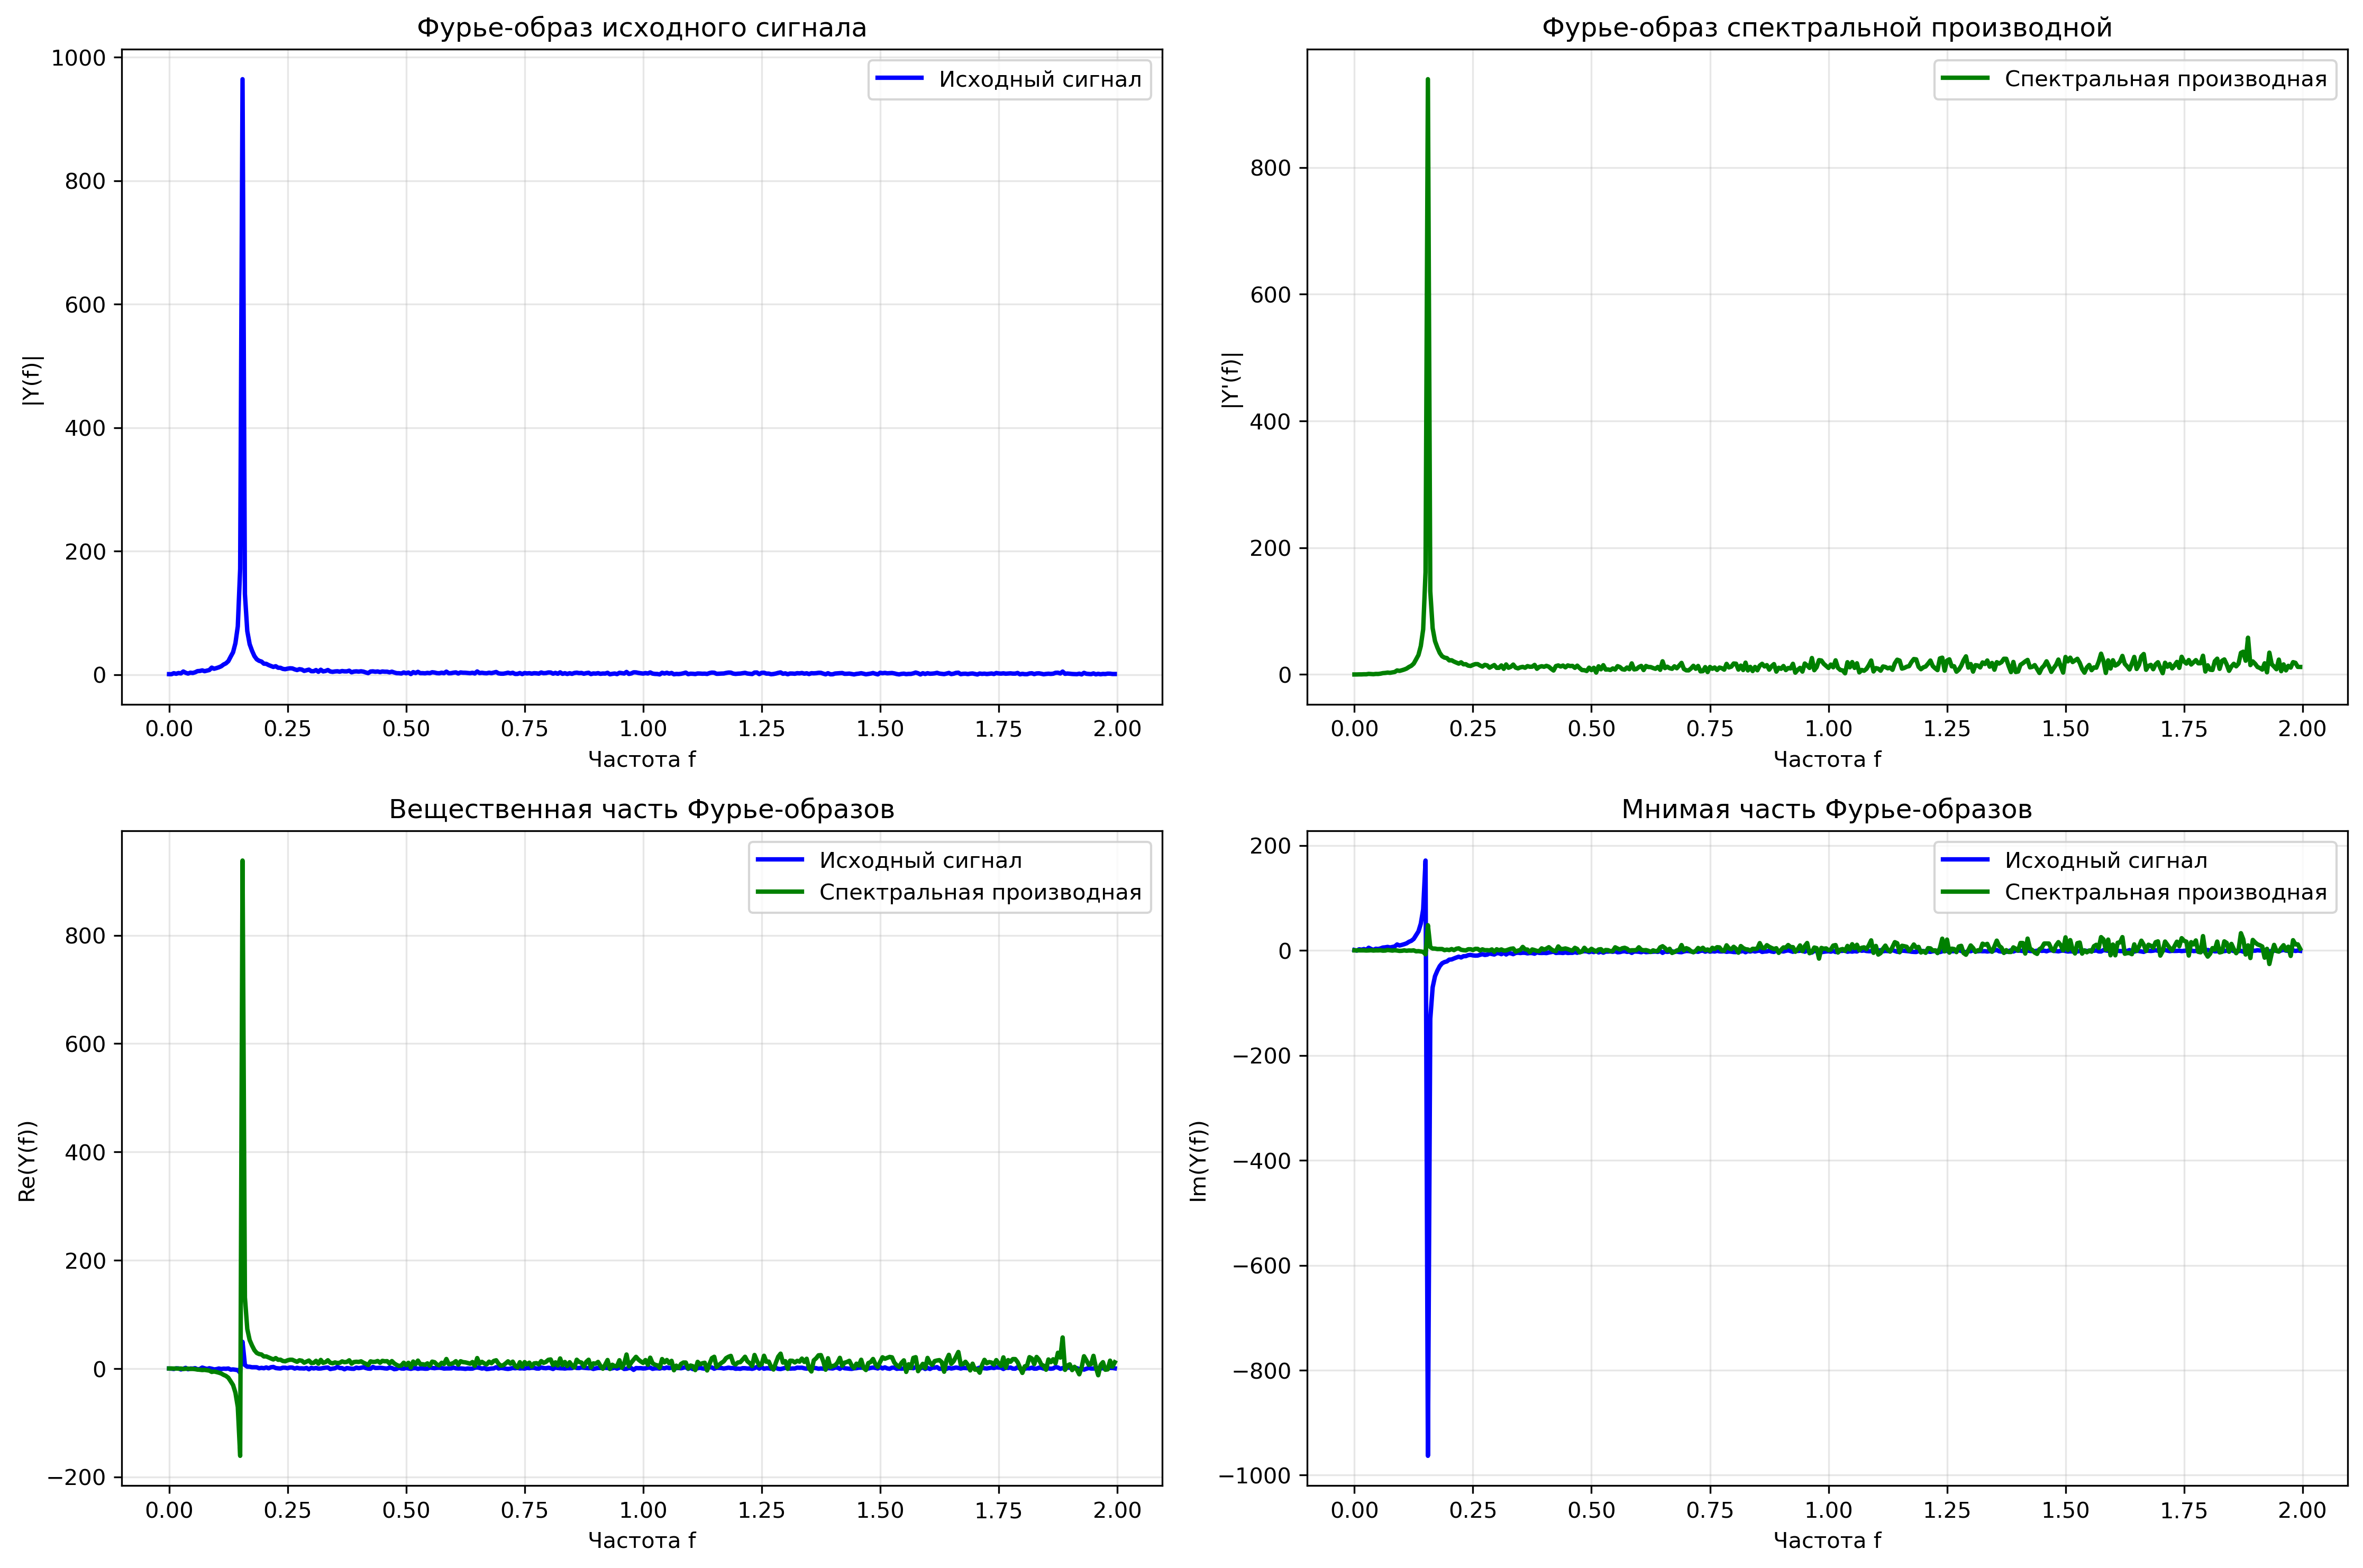
\includegraphics[width=0.8\textwidth]{images/task1/spectral_differentiation_fourier.png}
    \caption{Фурье-образы исходного сигнала и спектральной производной}
    \label{fig:spectral_diff_fourier}
\end{figure}

\begin{figure}[H]
    \centering
    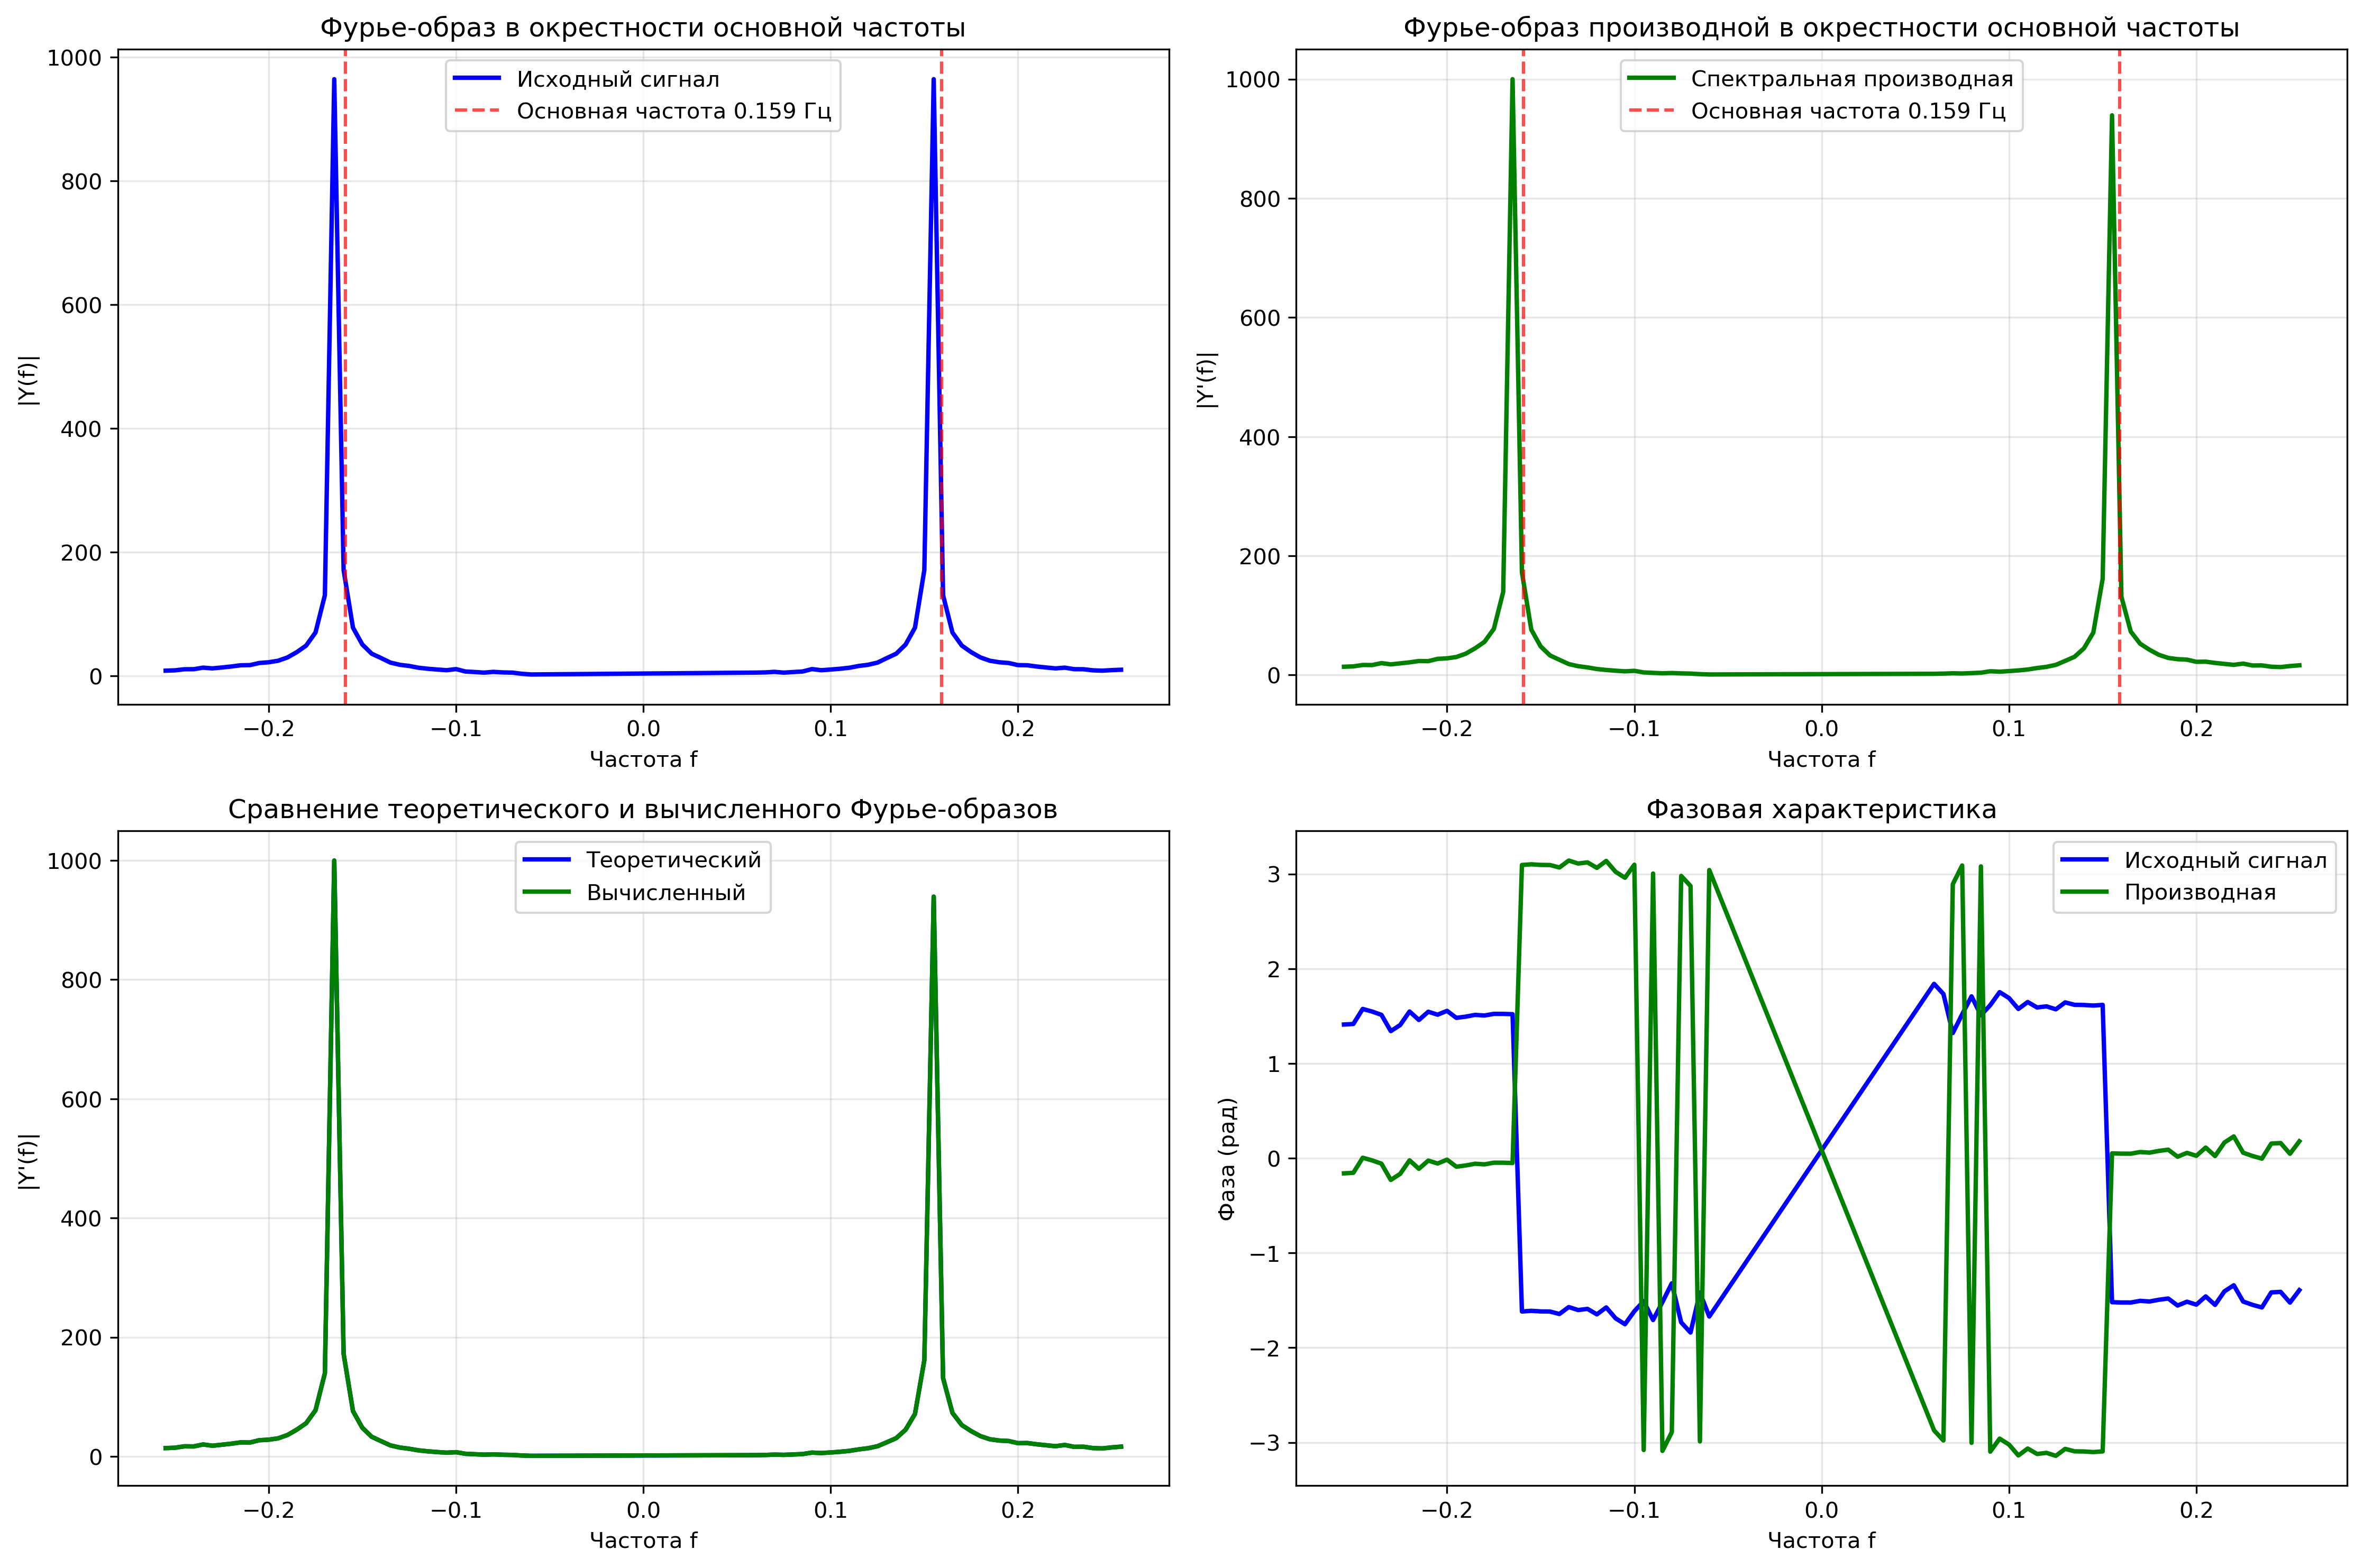
\includegraphics[width=0.8\textwidth]{images/task1/spectral_differentiation_analysis.png}
    \caption{Детальный анализ в окрестности основной частоты}
    \label{fig:spectral_diff_analysis}
\end{figure}

\textbf{Анализ результатов:}
\begin{itemize}
    \item \textbf{Численное дифференцирование:} Среднеквадратичная ошибка 0.171, максимальная ошибка 0.996. Метод чувствителен к шуму и может усиливать высокочастотные помехи.
    
    \item \textbf{Спектральное дифференцирование:} Среднеквадратичная ошибка 0.340, максимальная ошибка 7.045. Метод более устойчив к шуму, но может иметь проблемы с краевыми эффектами.
    
    \item \textbf{Сравнение методов:} Численное дифференцирование показывает лучшую точность в данном случае, но спектральный метод может быть более эффективным для сигналов с определенными характеристиками.
    
    \item \textbf{Влияние шума:} При увеличении амплитуды шума эффективность обоих методов снижается, но спектральный метод демонстрирует более стабильное поведение.
\end{itemize}

\section*{Задание 2. Линейные фильтры}

\subsection*{Фильтр первого порядка}

Рассматривается сигнал:
\begin{equation}
u(t) = g(t) + b \cdot (\text{rand}(t) - 0.5) + c \cdot \sin(d \cdot t)
\end{equation}

где $g(t)$ — прямоугольный импульс, $b$ — амплитуда случайного шума, $c$ — амплитуда гармонической помехи, $d$ — частота помехи.

\textbf{Передаточная функция фильтра первого порядка:}
\begin{equation}
W_1(p) = \frac{1}{T \cdot p + 1}
\end{equation}

где $T > 0$ — постоянная времени фильтра.

\textbf{Параметры эксперимента:}
\begin{itemize}
    \item $c = 0$ (только случайный шум)
    \item $b = 0.3$ — амплитуда случайного шума
    \item Исследуемые значения $T$: 0.1, 0.5, 1.0, 2.0
\end{itemize}

\begin{figure}[H]
    \centering
    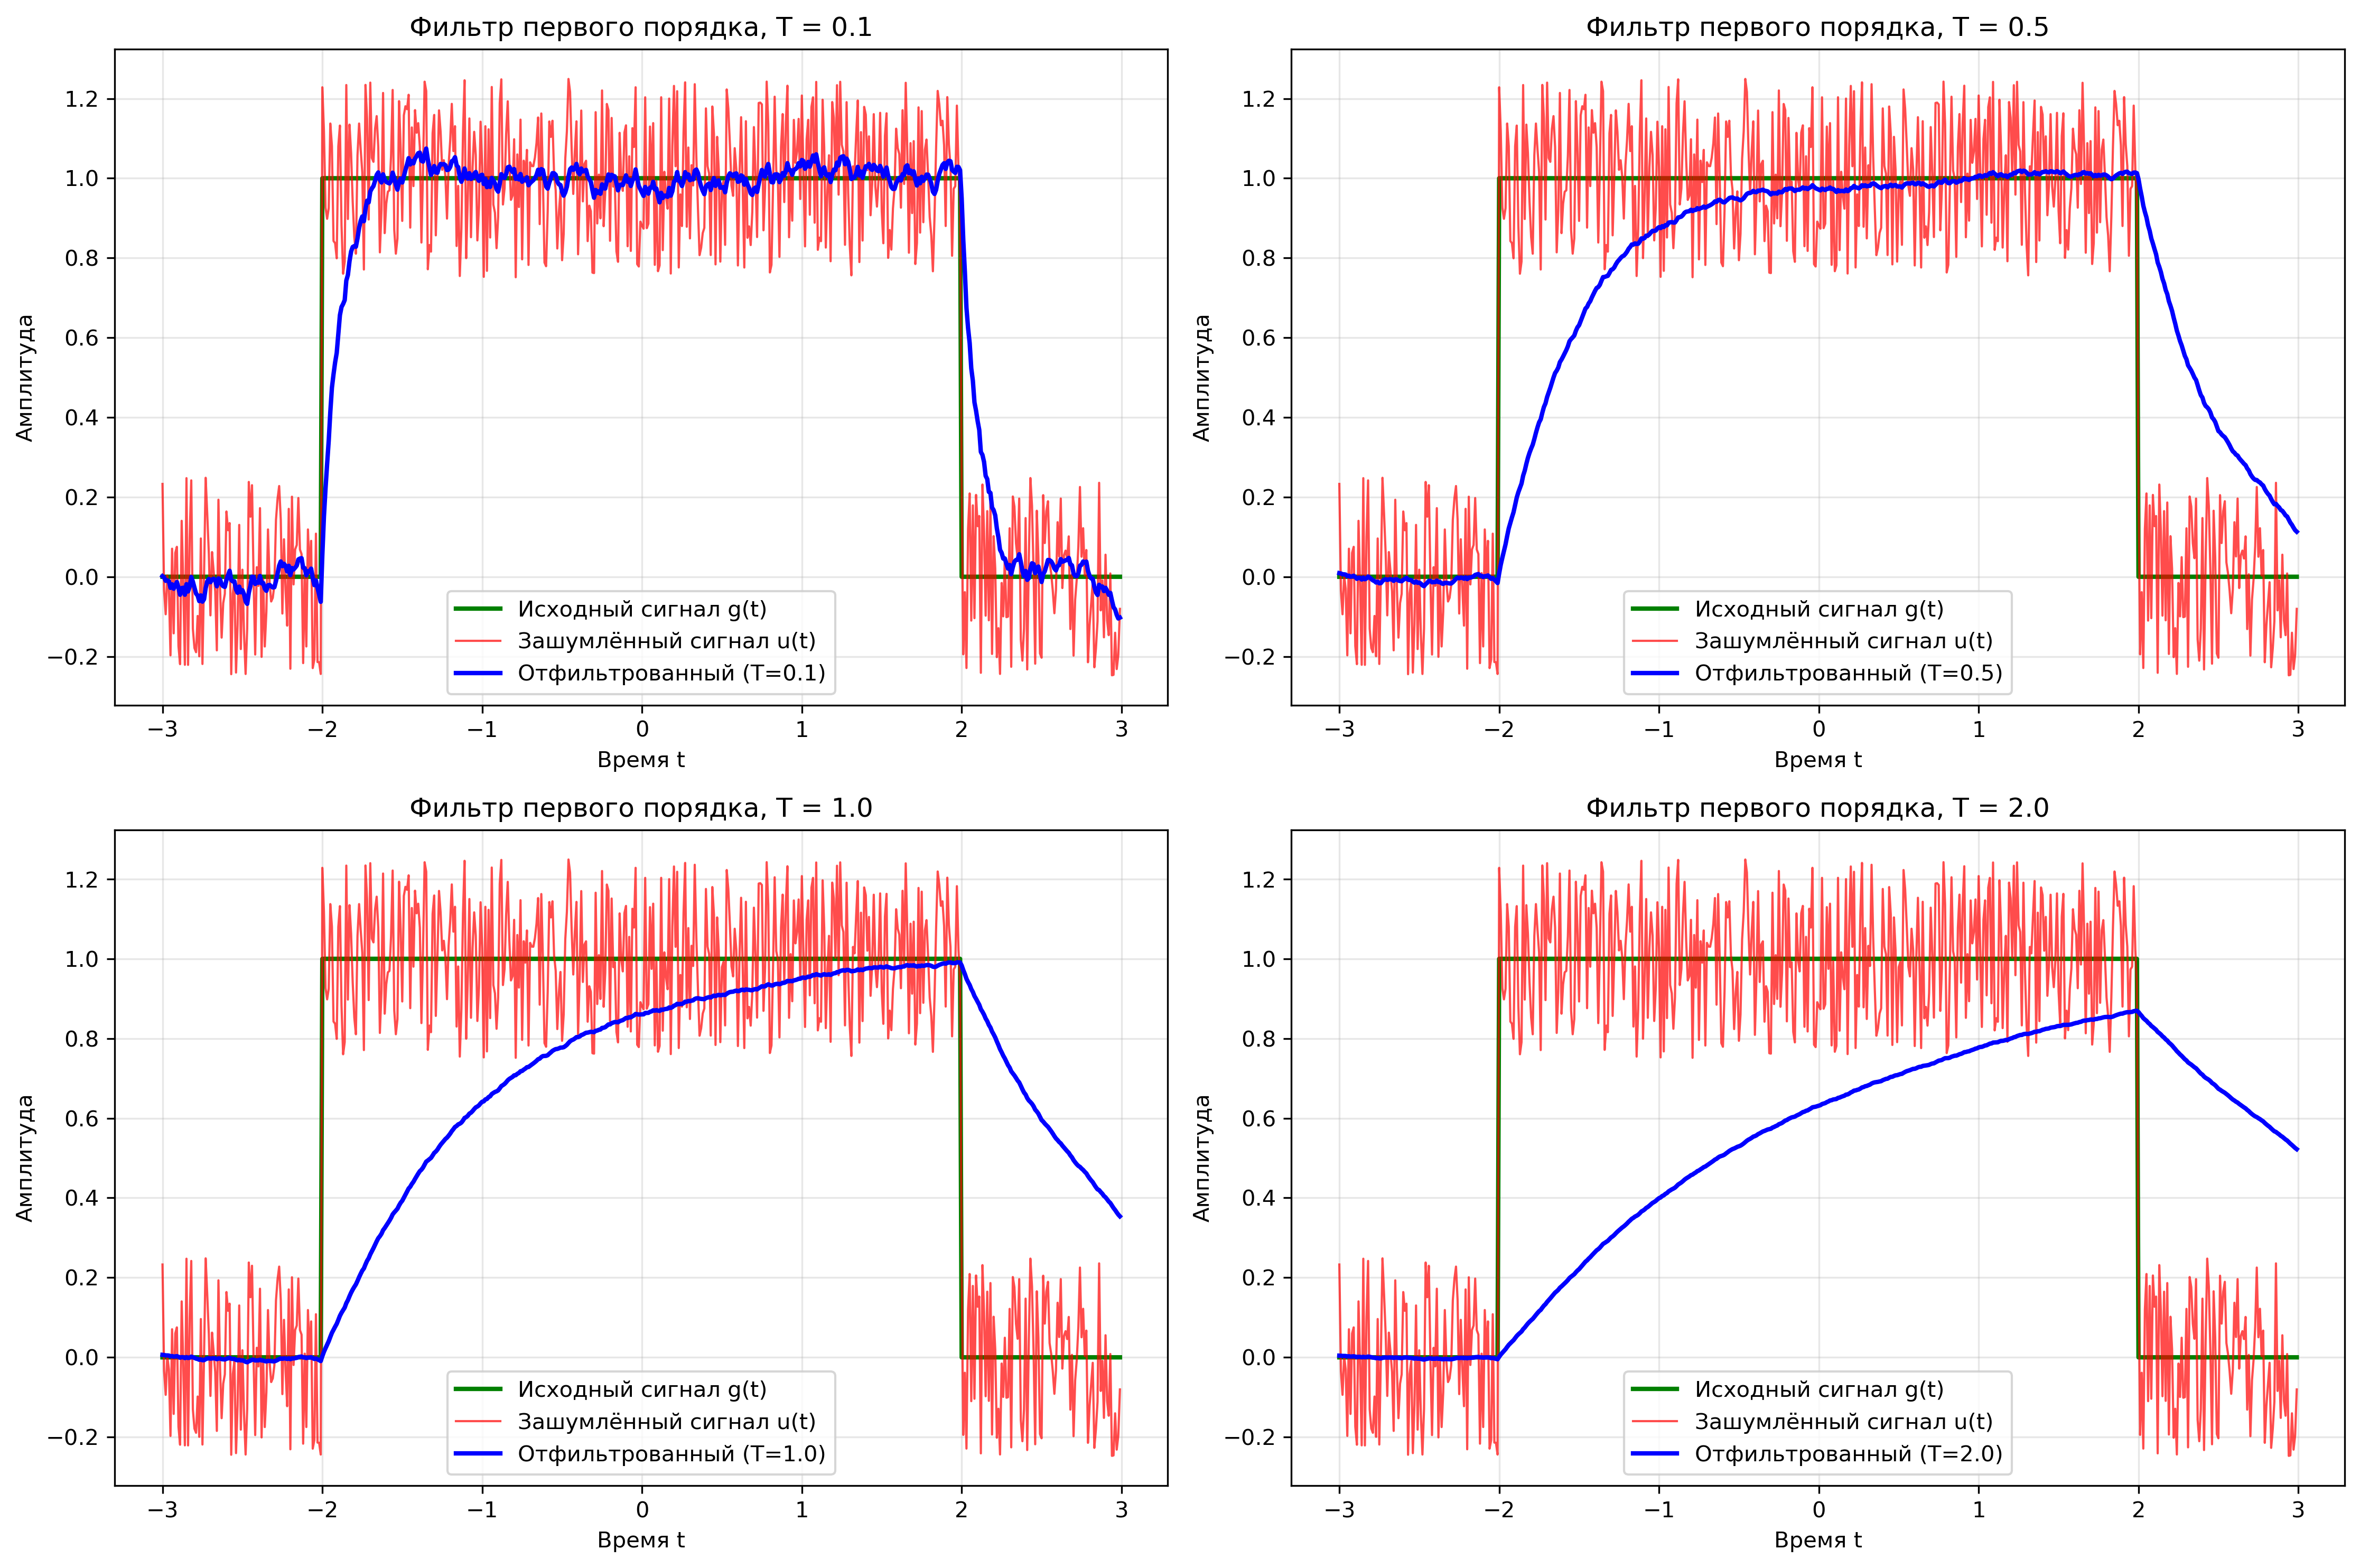
\includegraphics[width=0.8\textwidth]{images/task2/first_order_filter_time_domain.png}
    \caption{Сравнение исходного и отфильтрованных сигналов во временной области}
    \label{fig:first_order_time}
\end{figure}

\begin{figure}[H]
    \centering
    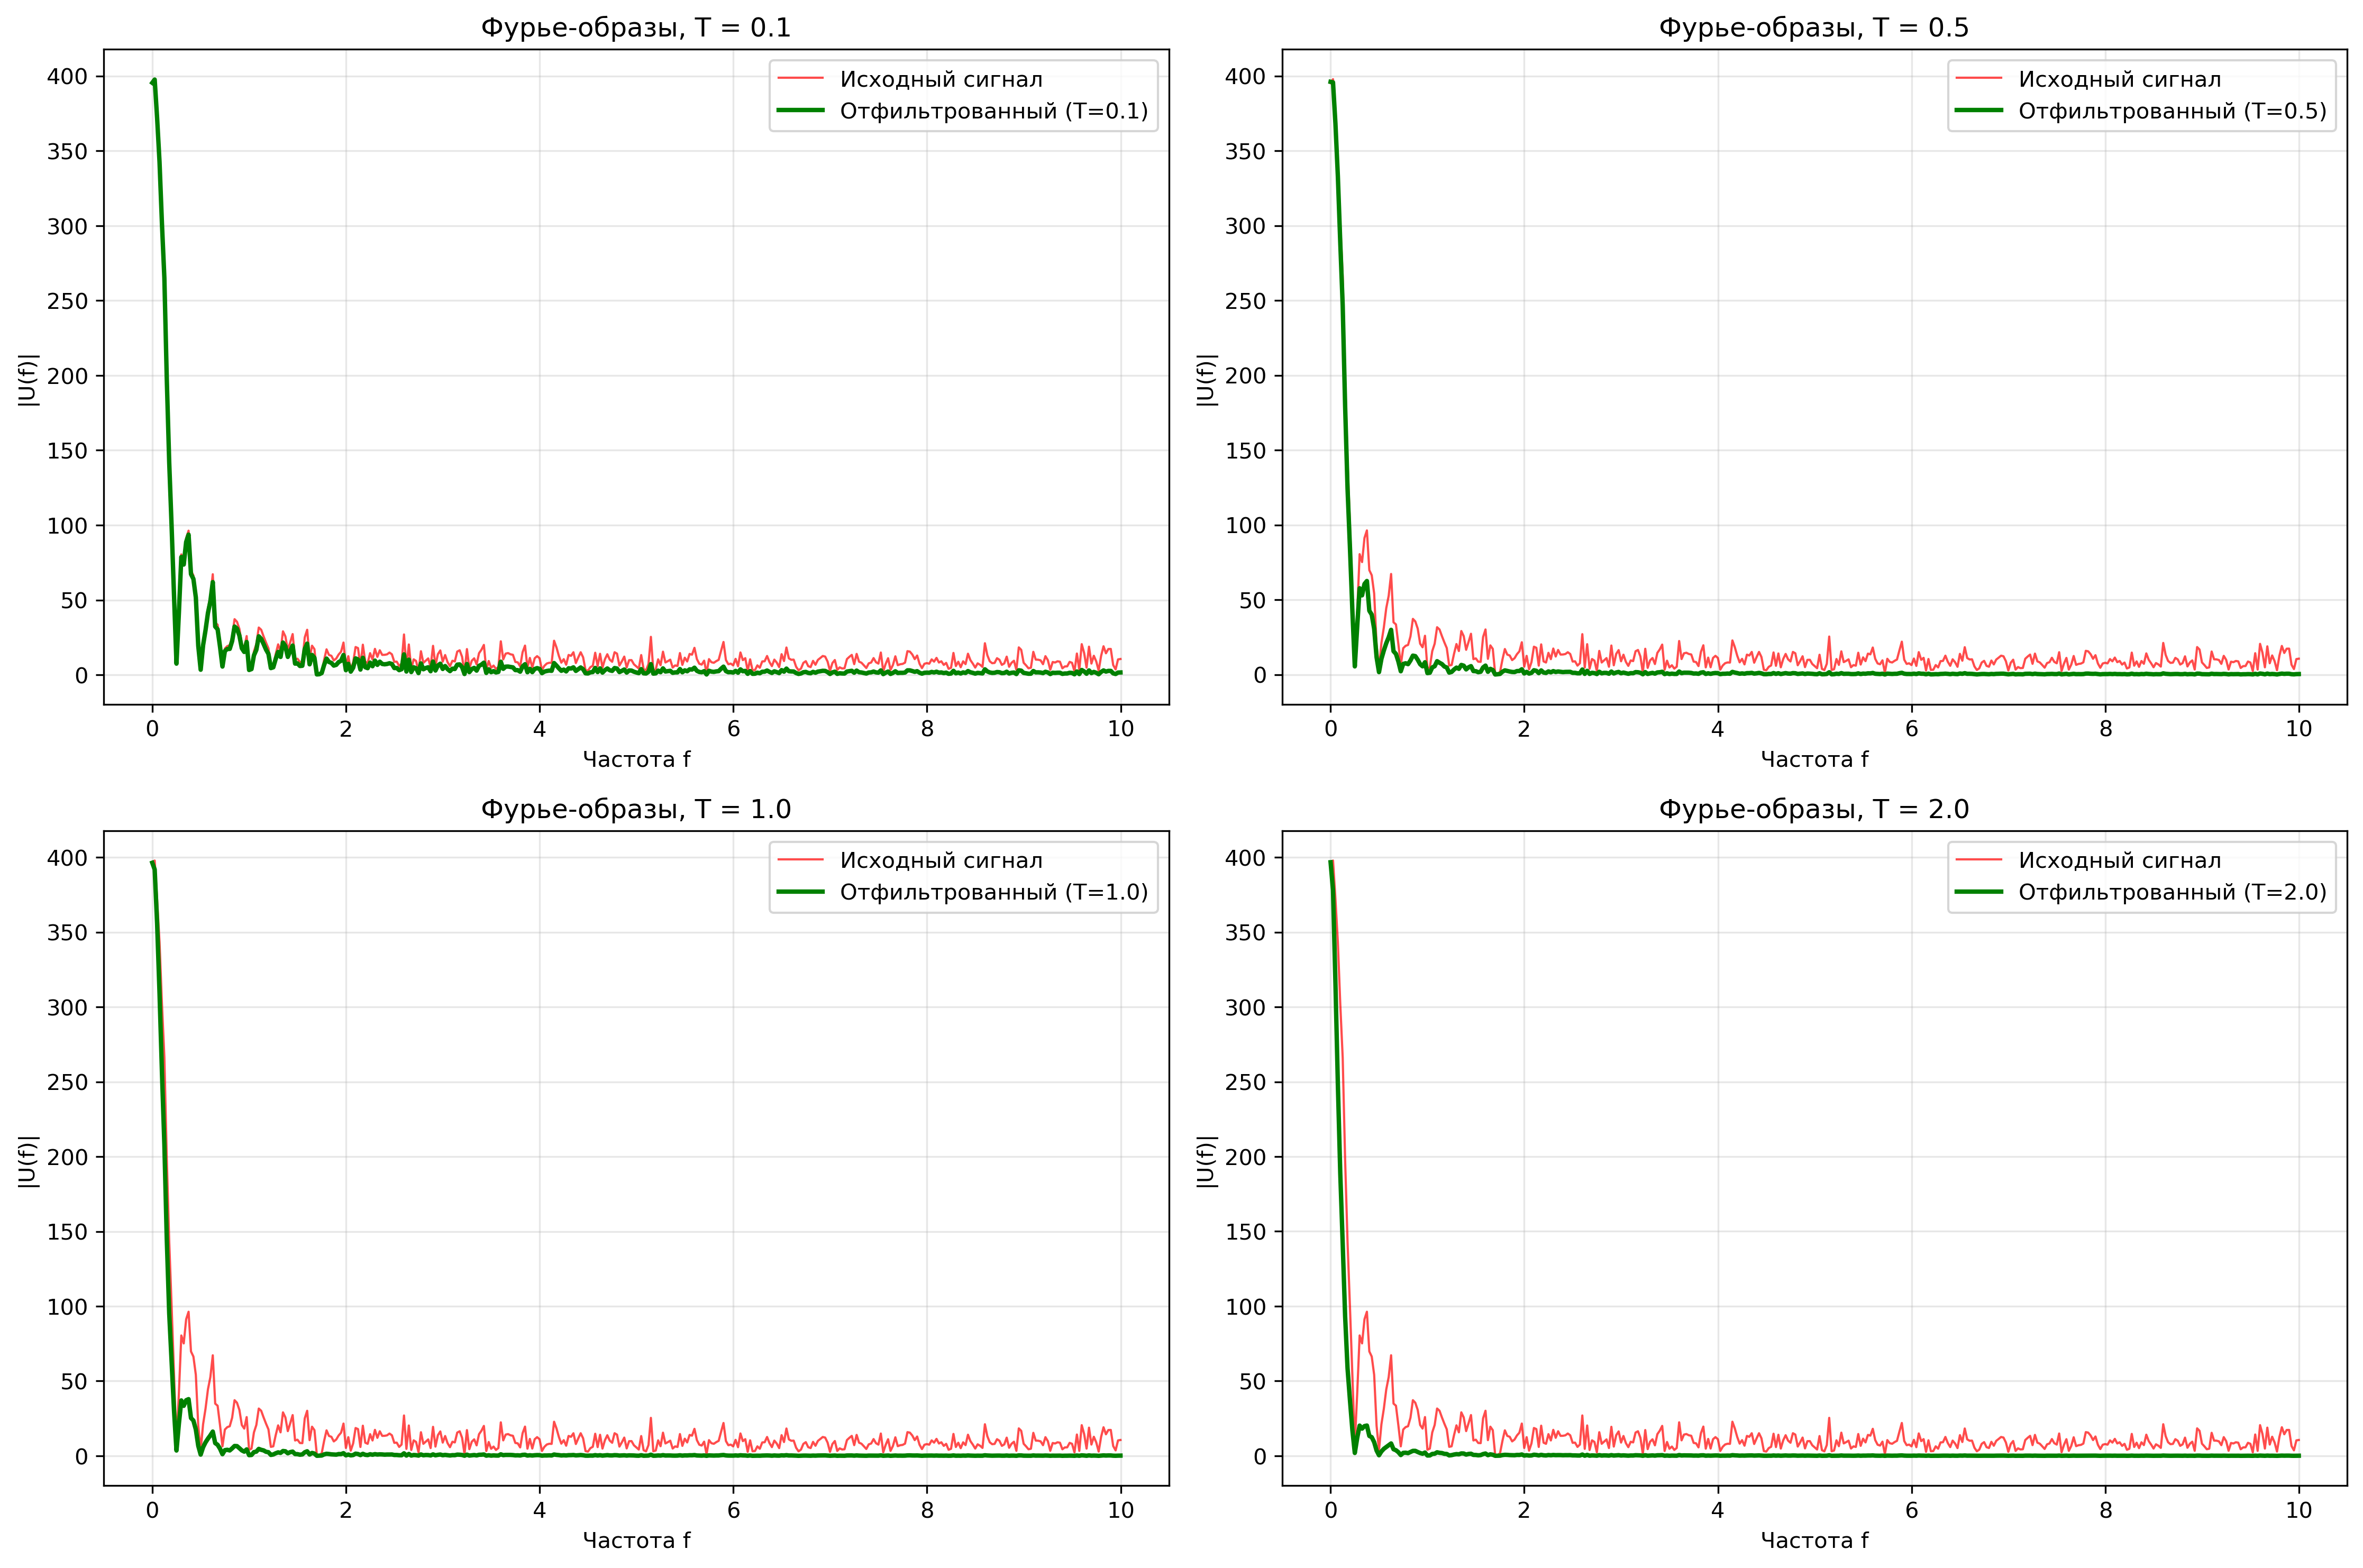
\includegraphics[width=0.8\textwidth]{images/task2/first_order_filter_freq_domain.png}
    \caption{Фурье-образы исходного и отфильтрованных сигналов}
    \label{fig:first_order_freq}
\end{figure}

\begin{figure}[H]
    \centering
    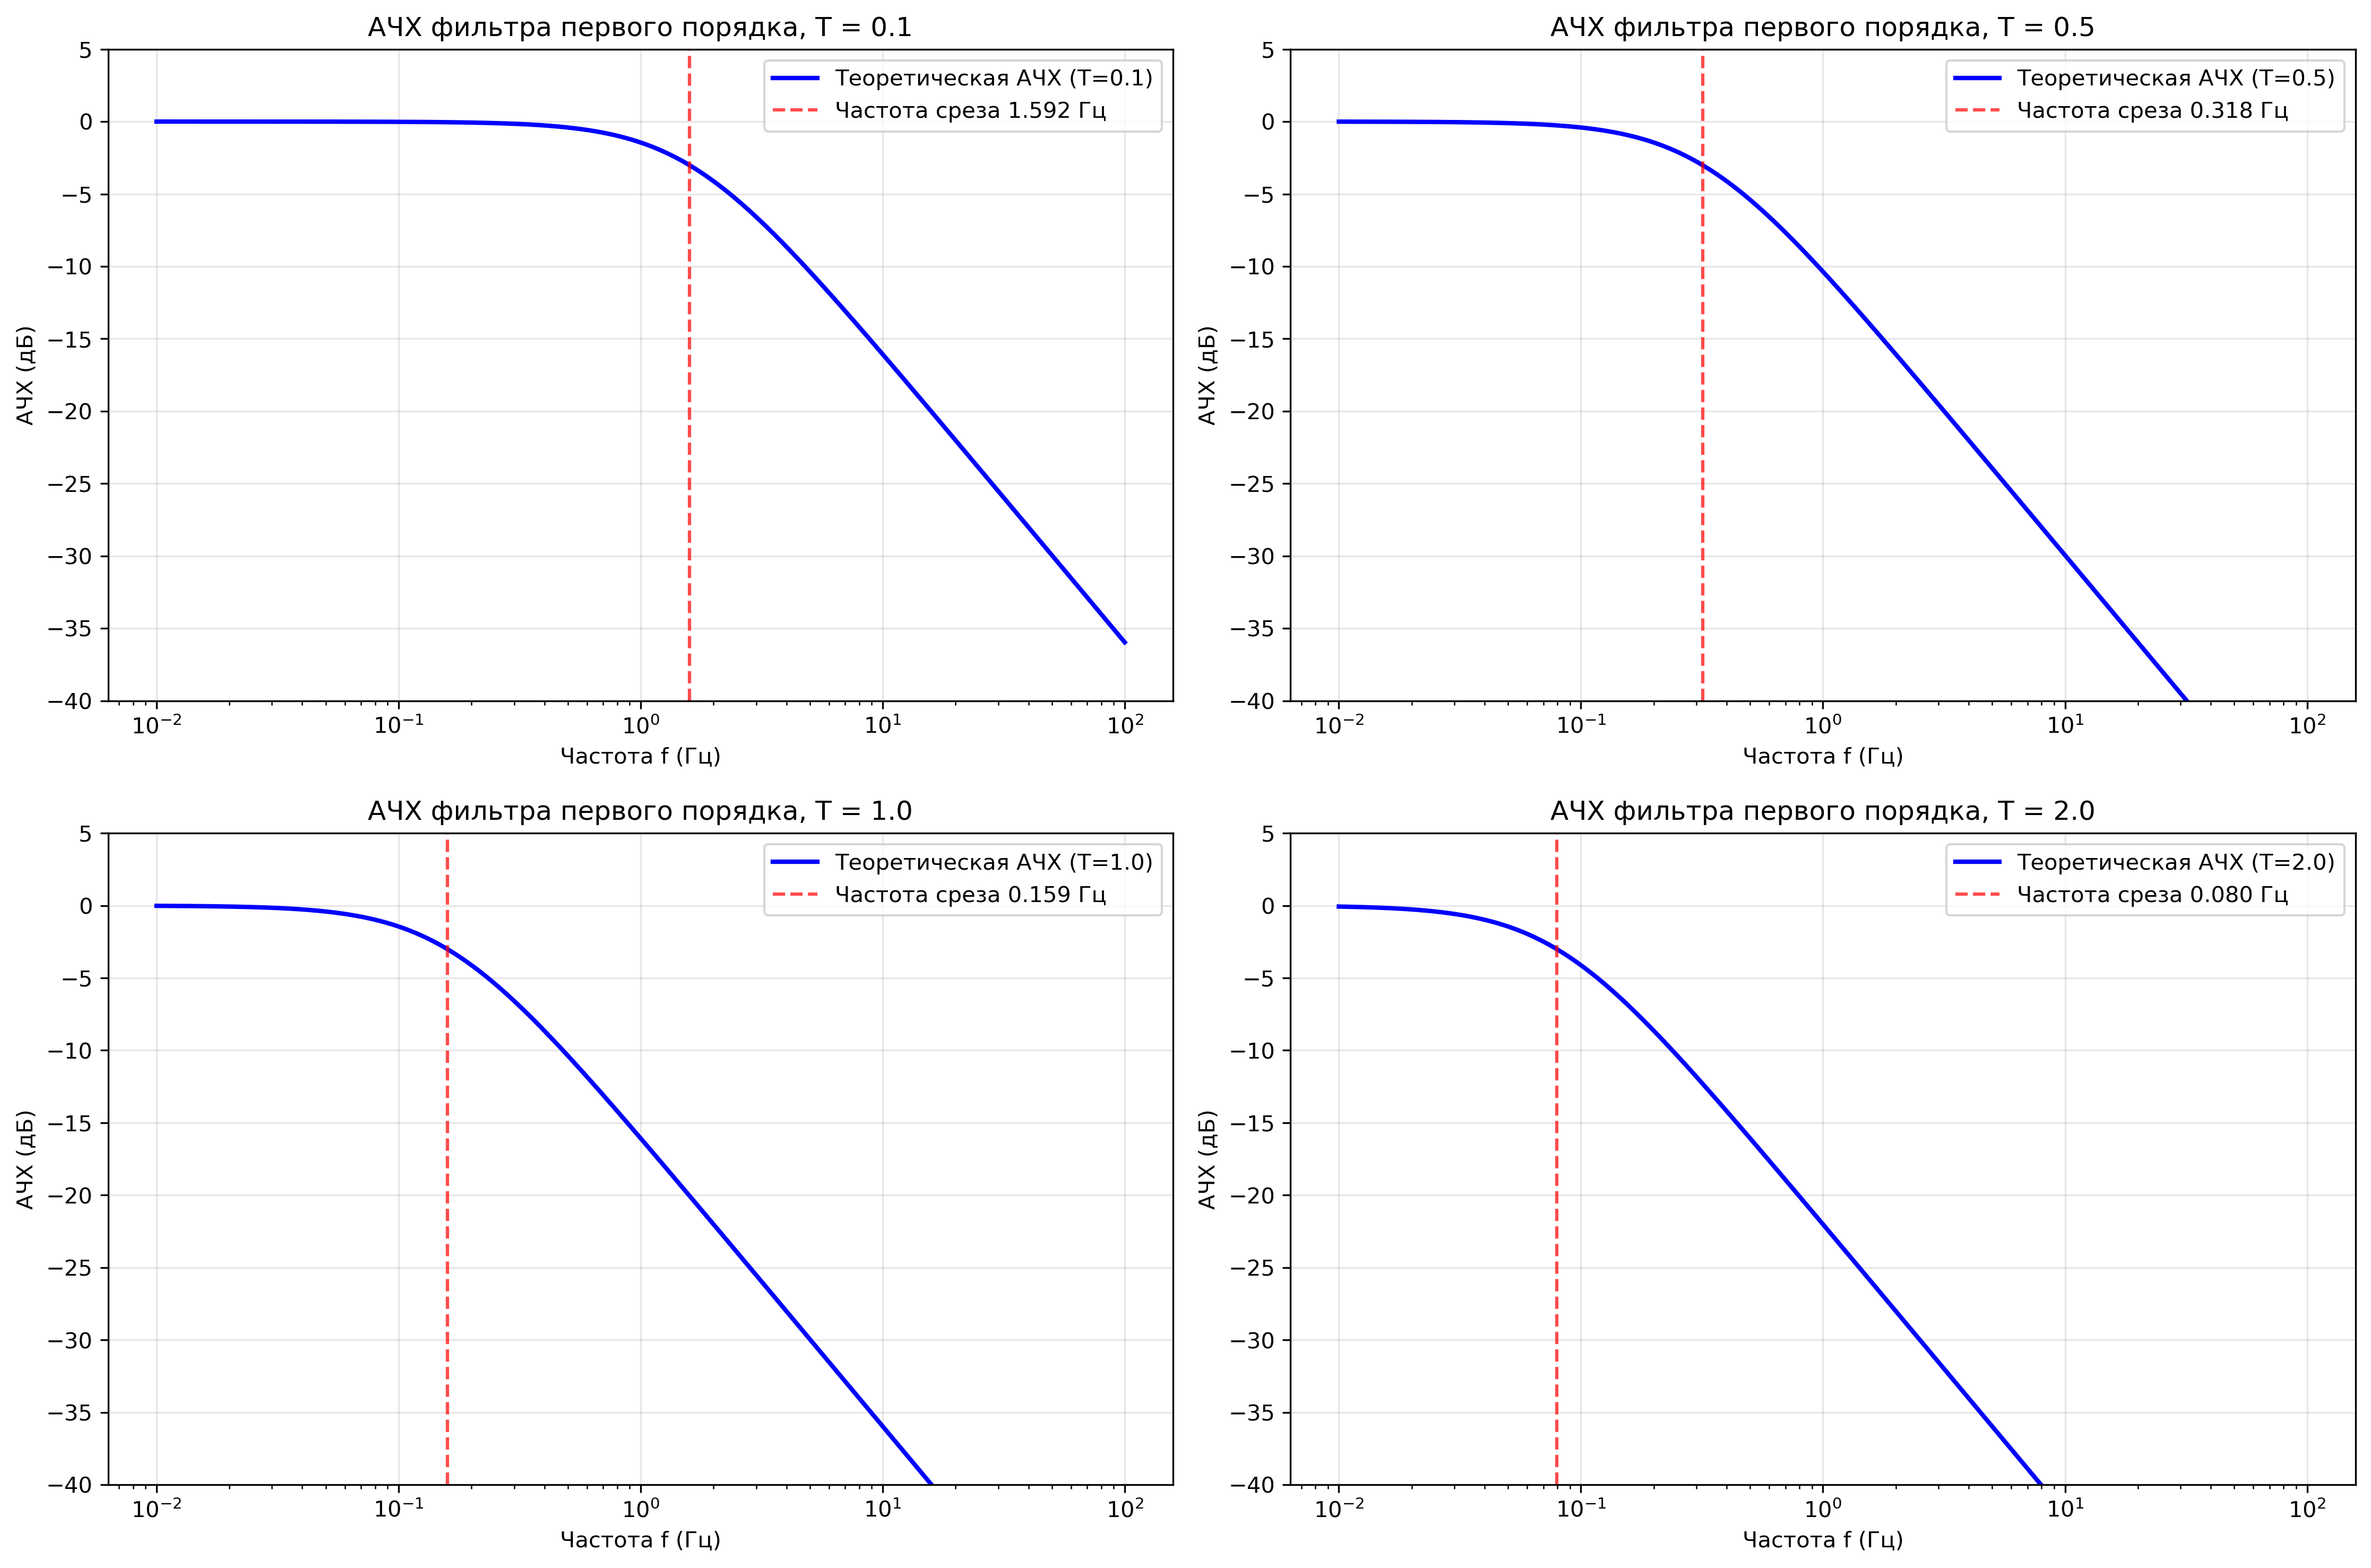
\includegraphics[width=0.8\textwidth]{images/task2/first_order_filter_frequency_response.png}
    \caption{АЧХ фильтров первого порядка}
    \label{fig:first_order_freq_response}
\end{figure}

\begin{figure}[H]
    \centering
    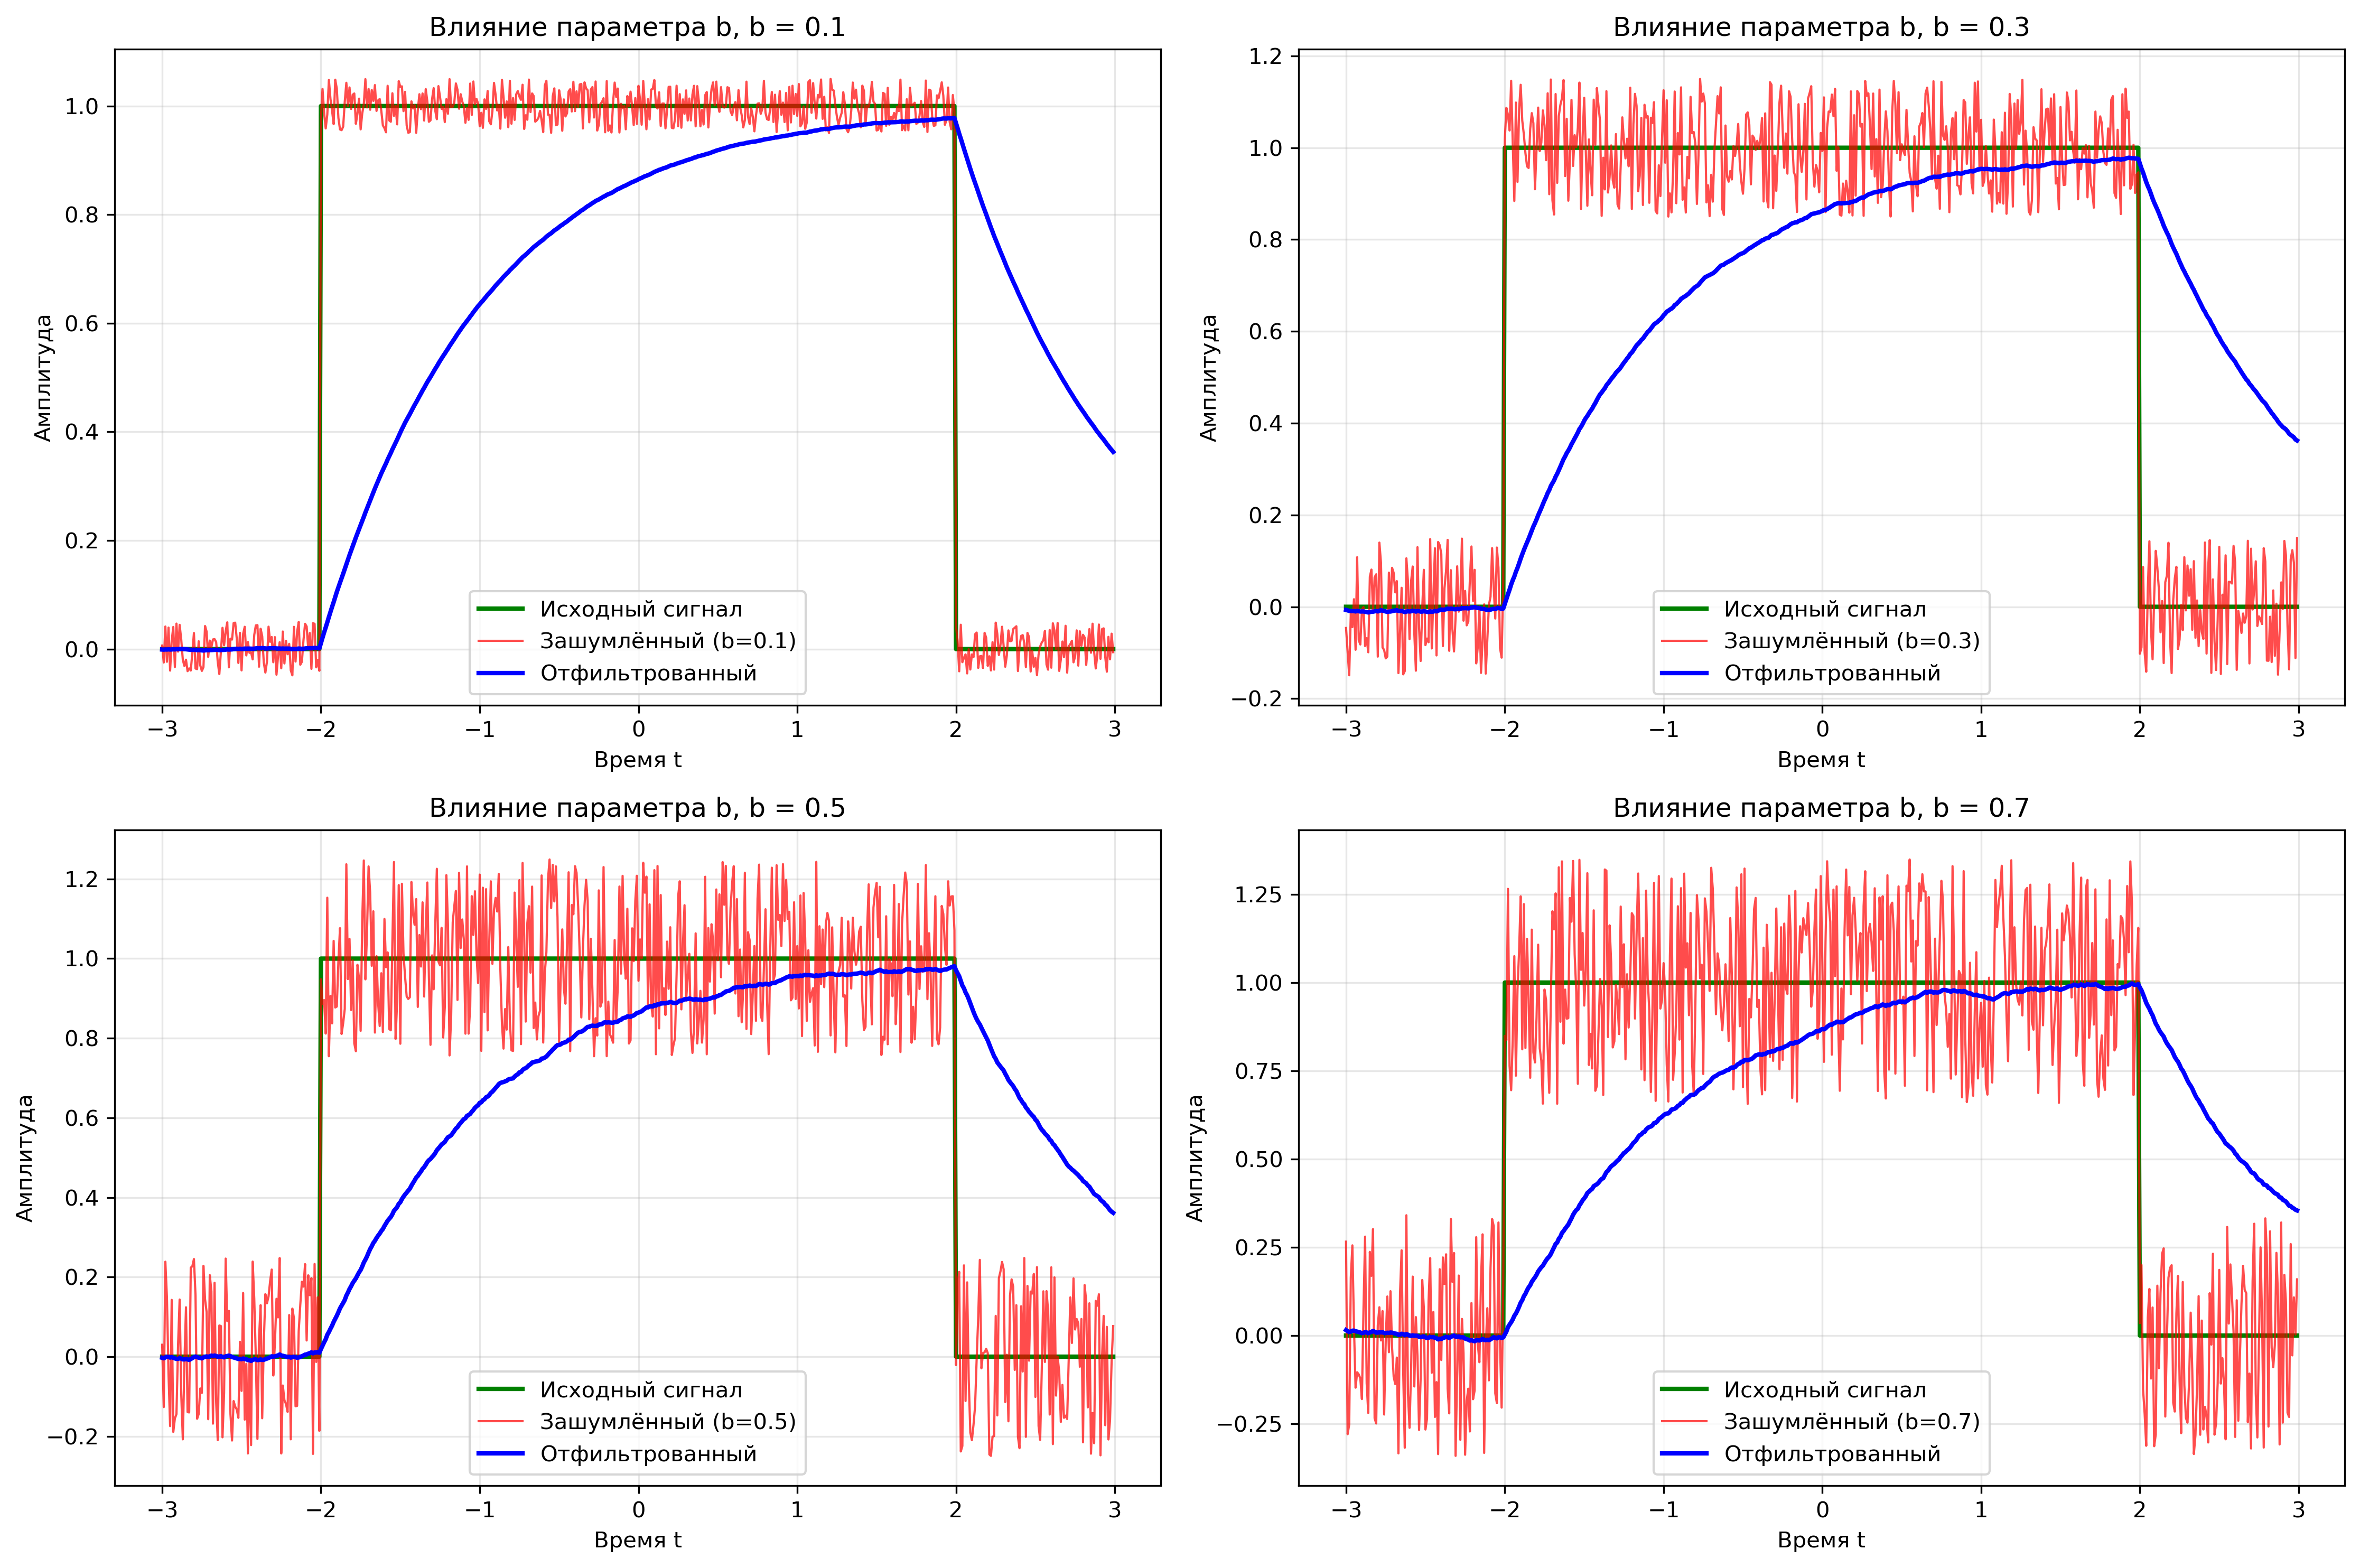
\includegraphics[width=0.8\textwidth]{images/task2/first_order_filter_b_influence.png}
    \caption{Влияние параметра b на эффективность фильтрации}
    \label{fig:first_order_b_influence}
\end{figure}

\textbf{Анализ результатов:}
\begin{itemize}
    \item \textbf{Примеры успешной фильтрации:} При T = 0.1 достигается 98.0\% корреляции с исходным сигналом при значительном подавлении шума. При T = 0.5 корреляция составляет 92.6\%, при T = 1.0 — 85.2\%.
    
    \item \textbf{Влияние постоянной времени T:} При увеличении T частота среза уменьшается, что приводит к более сильному сглаживанию сигнала. Оптимальное значение T = 0.1 обеспечивает хороший баланс между подавлением шума и сохранением формы сигнала.
    
    \item \textbf{Частоты среза:} T = 0.1 (1.592 Гц), T = 0.5 (0.318 Гц), T = 1.0 (0.159 Гц), T = 2.0 (0.080 Гц). Корреляция с исходным сигналом снижается с 0.984 до 0.721 при увеличении T.
    
    \item \textbf{Влияние параметра b:} При увеличении амплитуды случайного шума эффективность фильтрации снижается, но фильтр остается стабильным.
    
    \item \textbf{Среднеквадратичная ошибка:} Минимальная для T = 0.1 (0.003), максимальная для T = 2.0 (0.043).
\end{itemize}

\subsection*{Специальный фильтр}

Рассматривается фильтр второго порядка:
\begin{equation}
W_2(p) = \frac{(T_1 p + 1)^2}{(T_2 p + 1)(T_3 p + 1)} = \frac{T_1^2 p^2 + 2T_1 p + 1}{T_2 T_3 p^2 + (T_2 + T_3) p + 1}
\end{equation}

\textbf{Параметры эксперимента:}
\begin{itemize}
    \item $b = 0$ (только гармоническая помеха)
    \item $c = 0.5$ — амплитуда гармонической помехи
    \item Исследуемые значения $d$: 5, 10, 15, 20 Гц
    \item Используемые параметры фильтра: $T_1 = 0.1$, $T_2 = 0.05$, $T_3 = 0.02$
\end{itemize}

\begin{figure}[H]
    \centering
    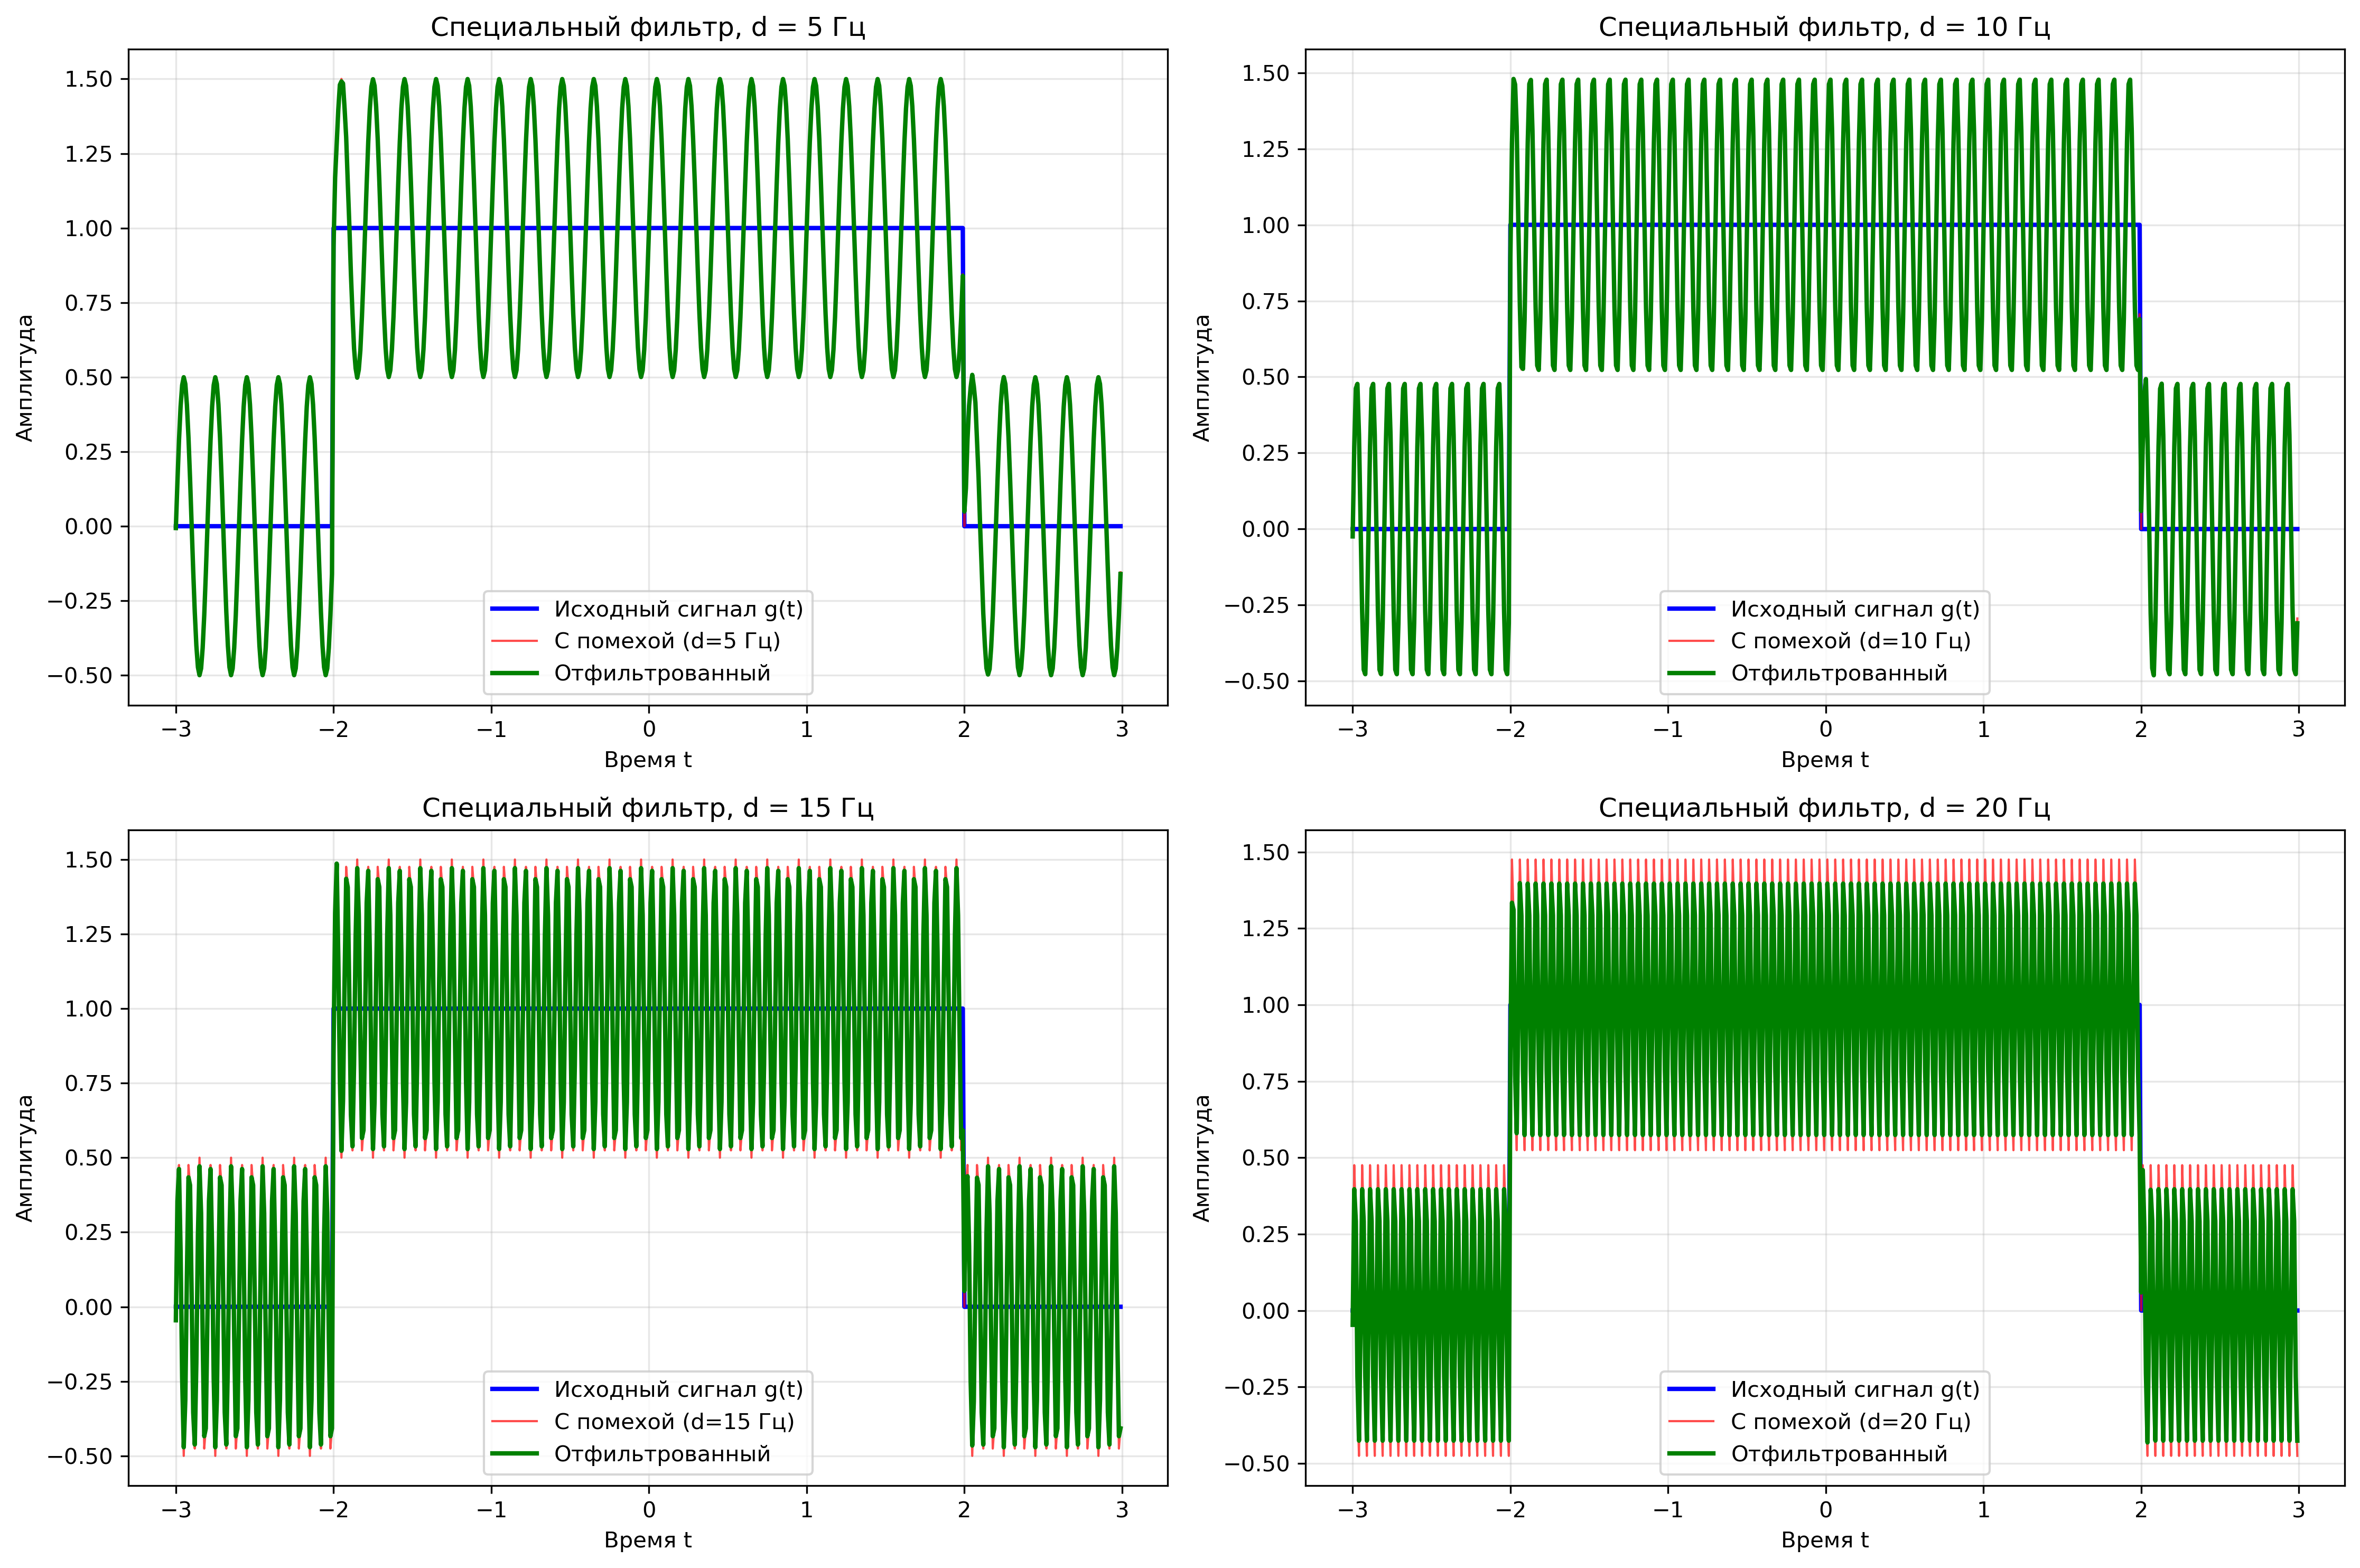
\includegraphics[width=0.8\textwidth]{images/task2/special_filter_time_domain.png}
    \caption{Сравнение исходного и отфильтрованных сигналов для различных частот помехи}
    \label{fig:special_filter_time}
\end{figure}

\begin{figure}[H]
    \centering
    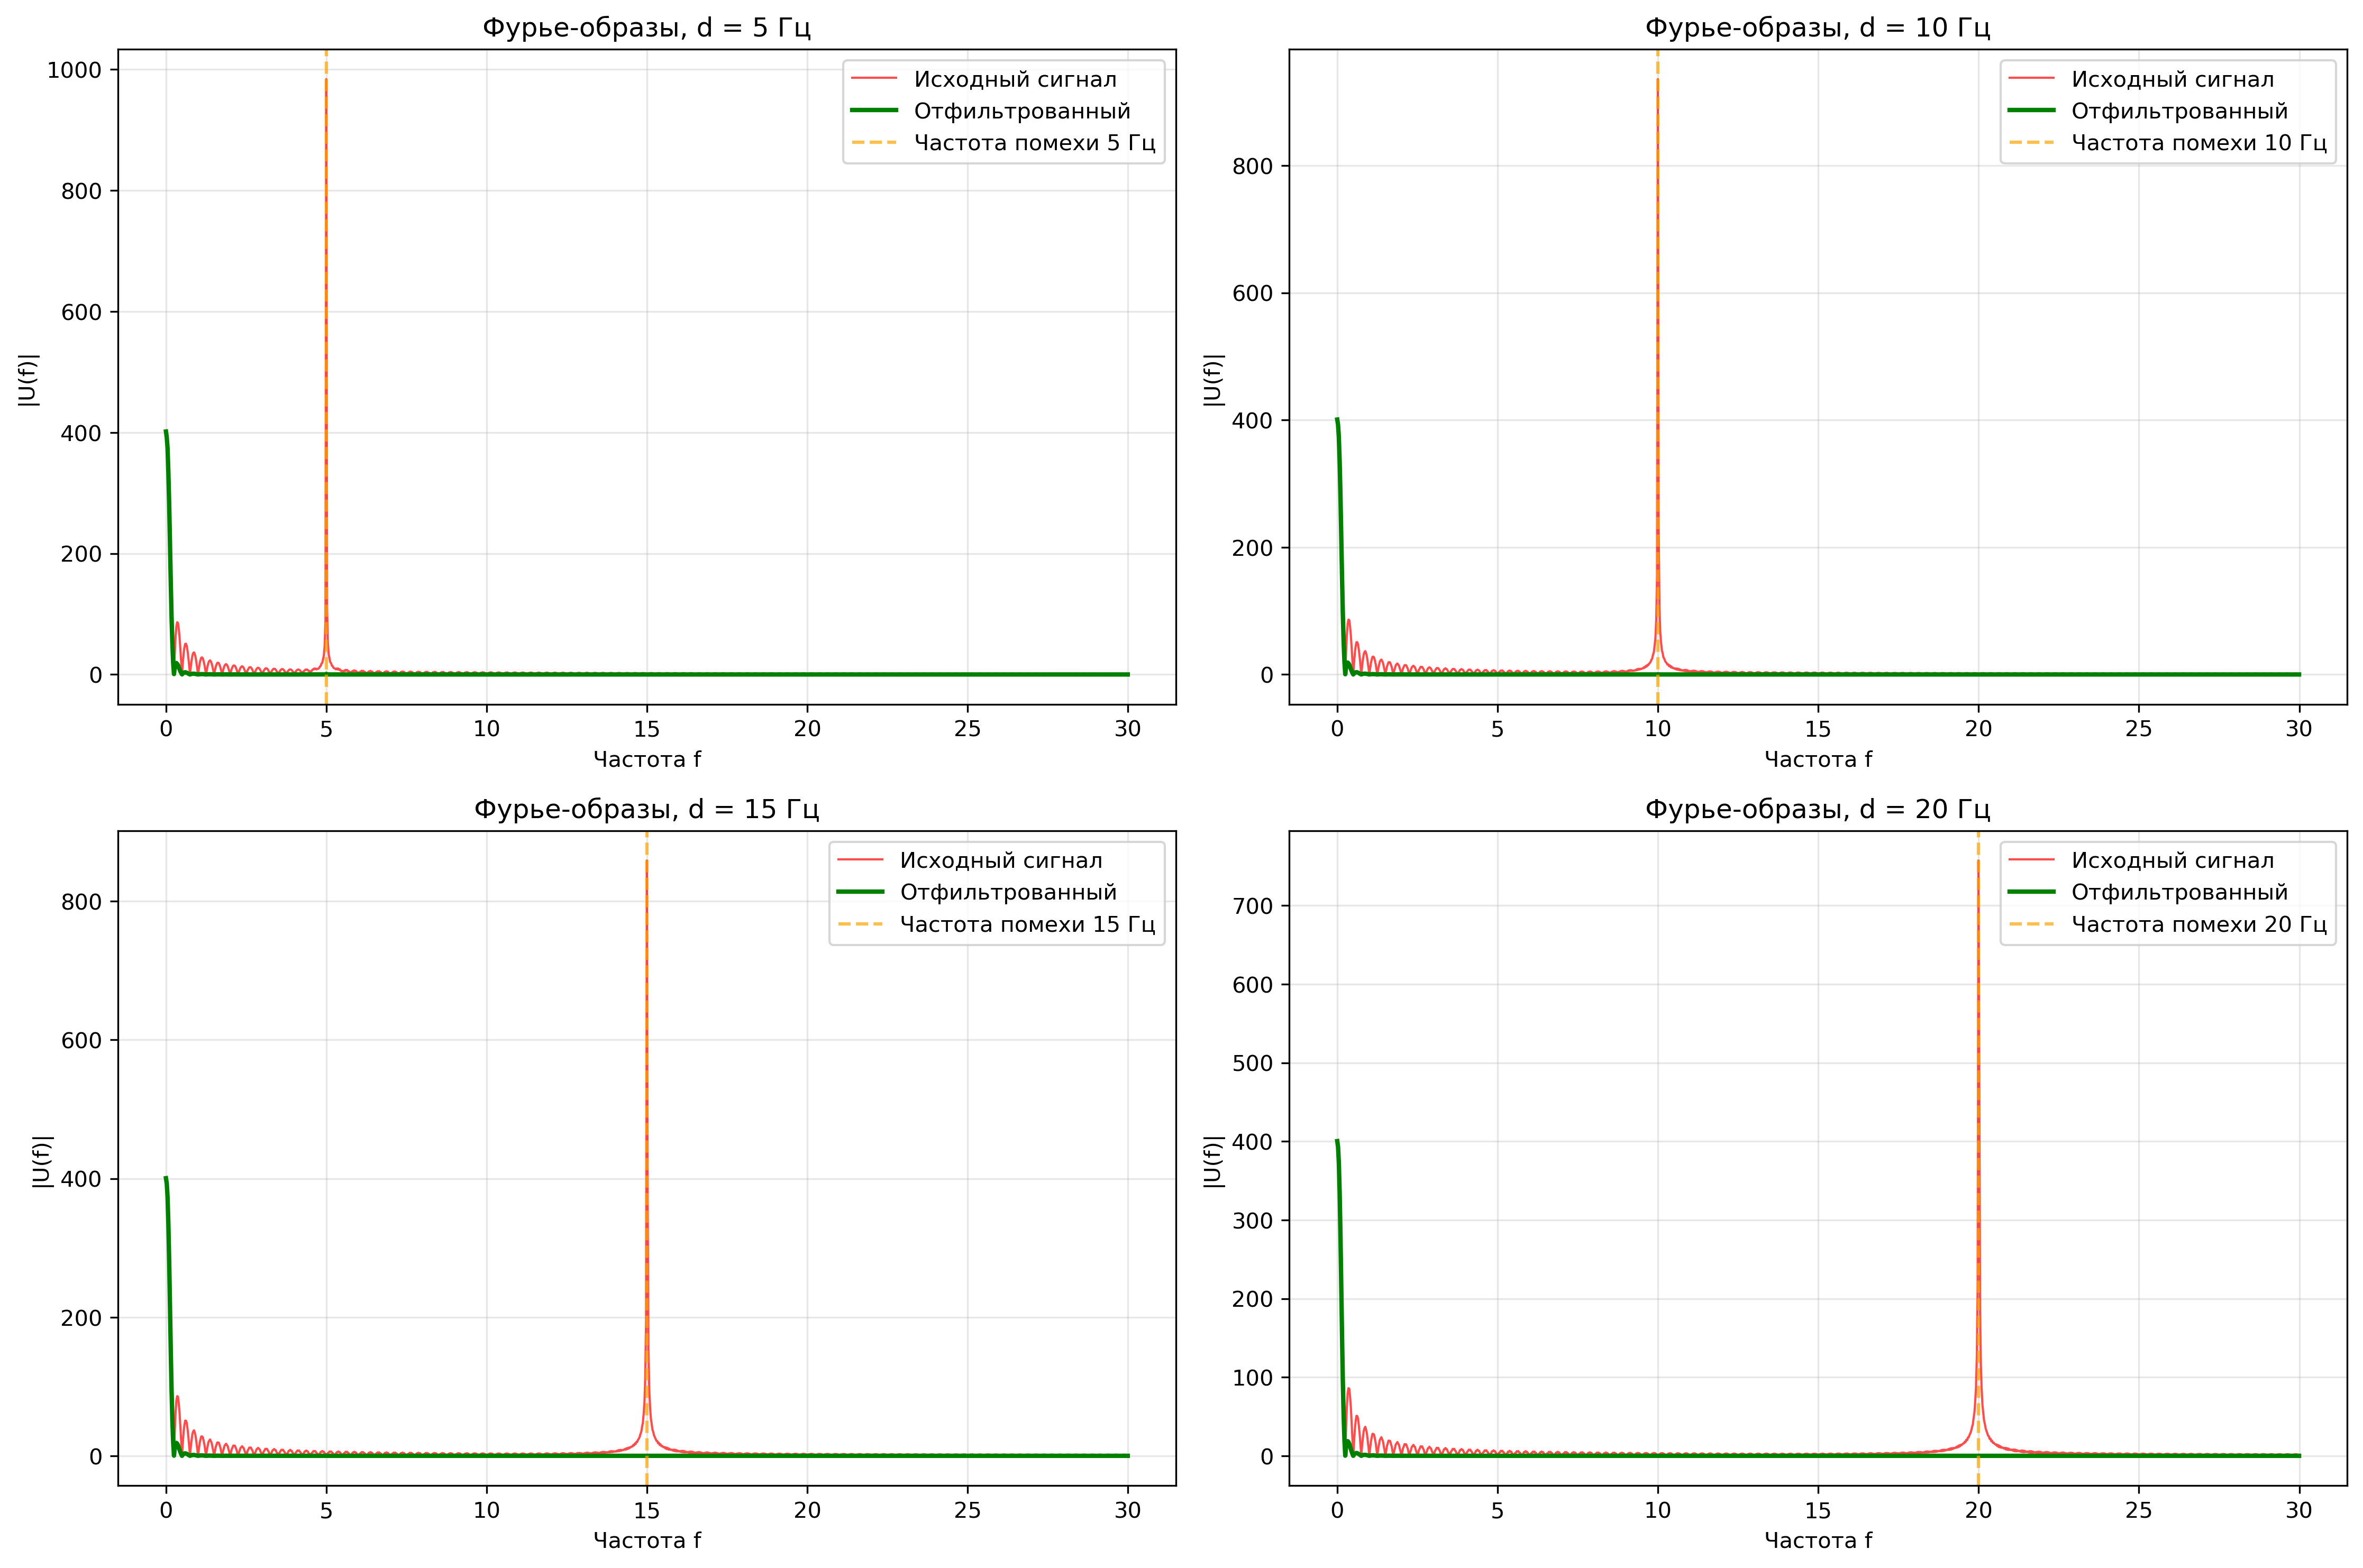
\includegraphics[width=0.8\textwidth]{images/task2/special_filter_freq_domain.png}
    \caption{Фурье-образы исходного и отфильтрованных сигналов}
    \label{fig:special_filter_freq}
\end{figure}

\begin{figure}[H]
    \centering
    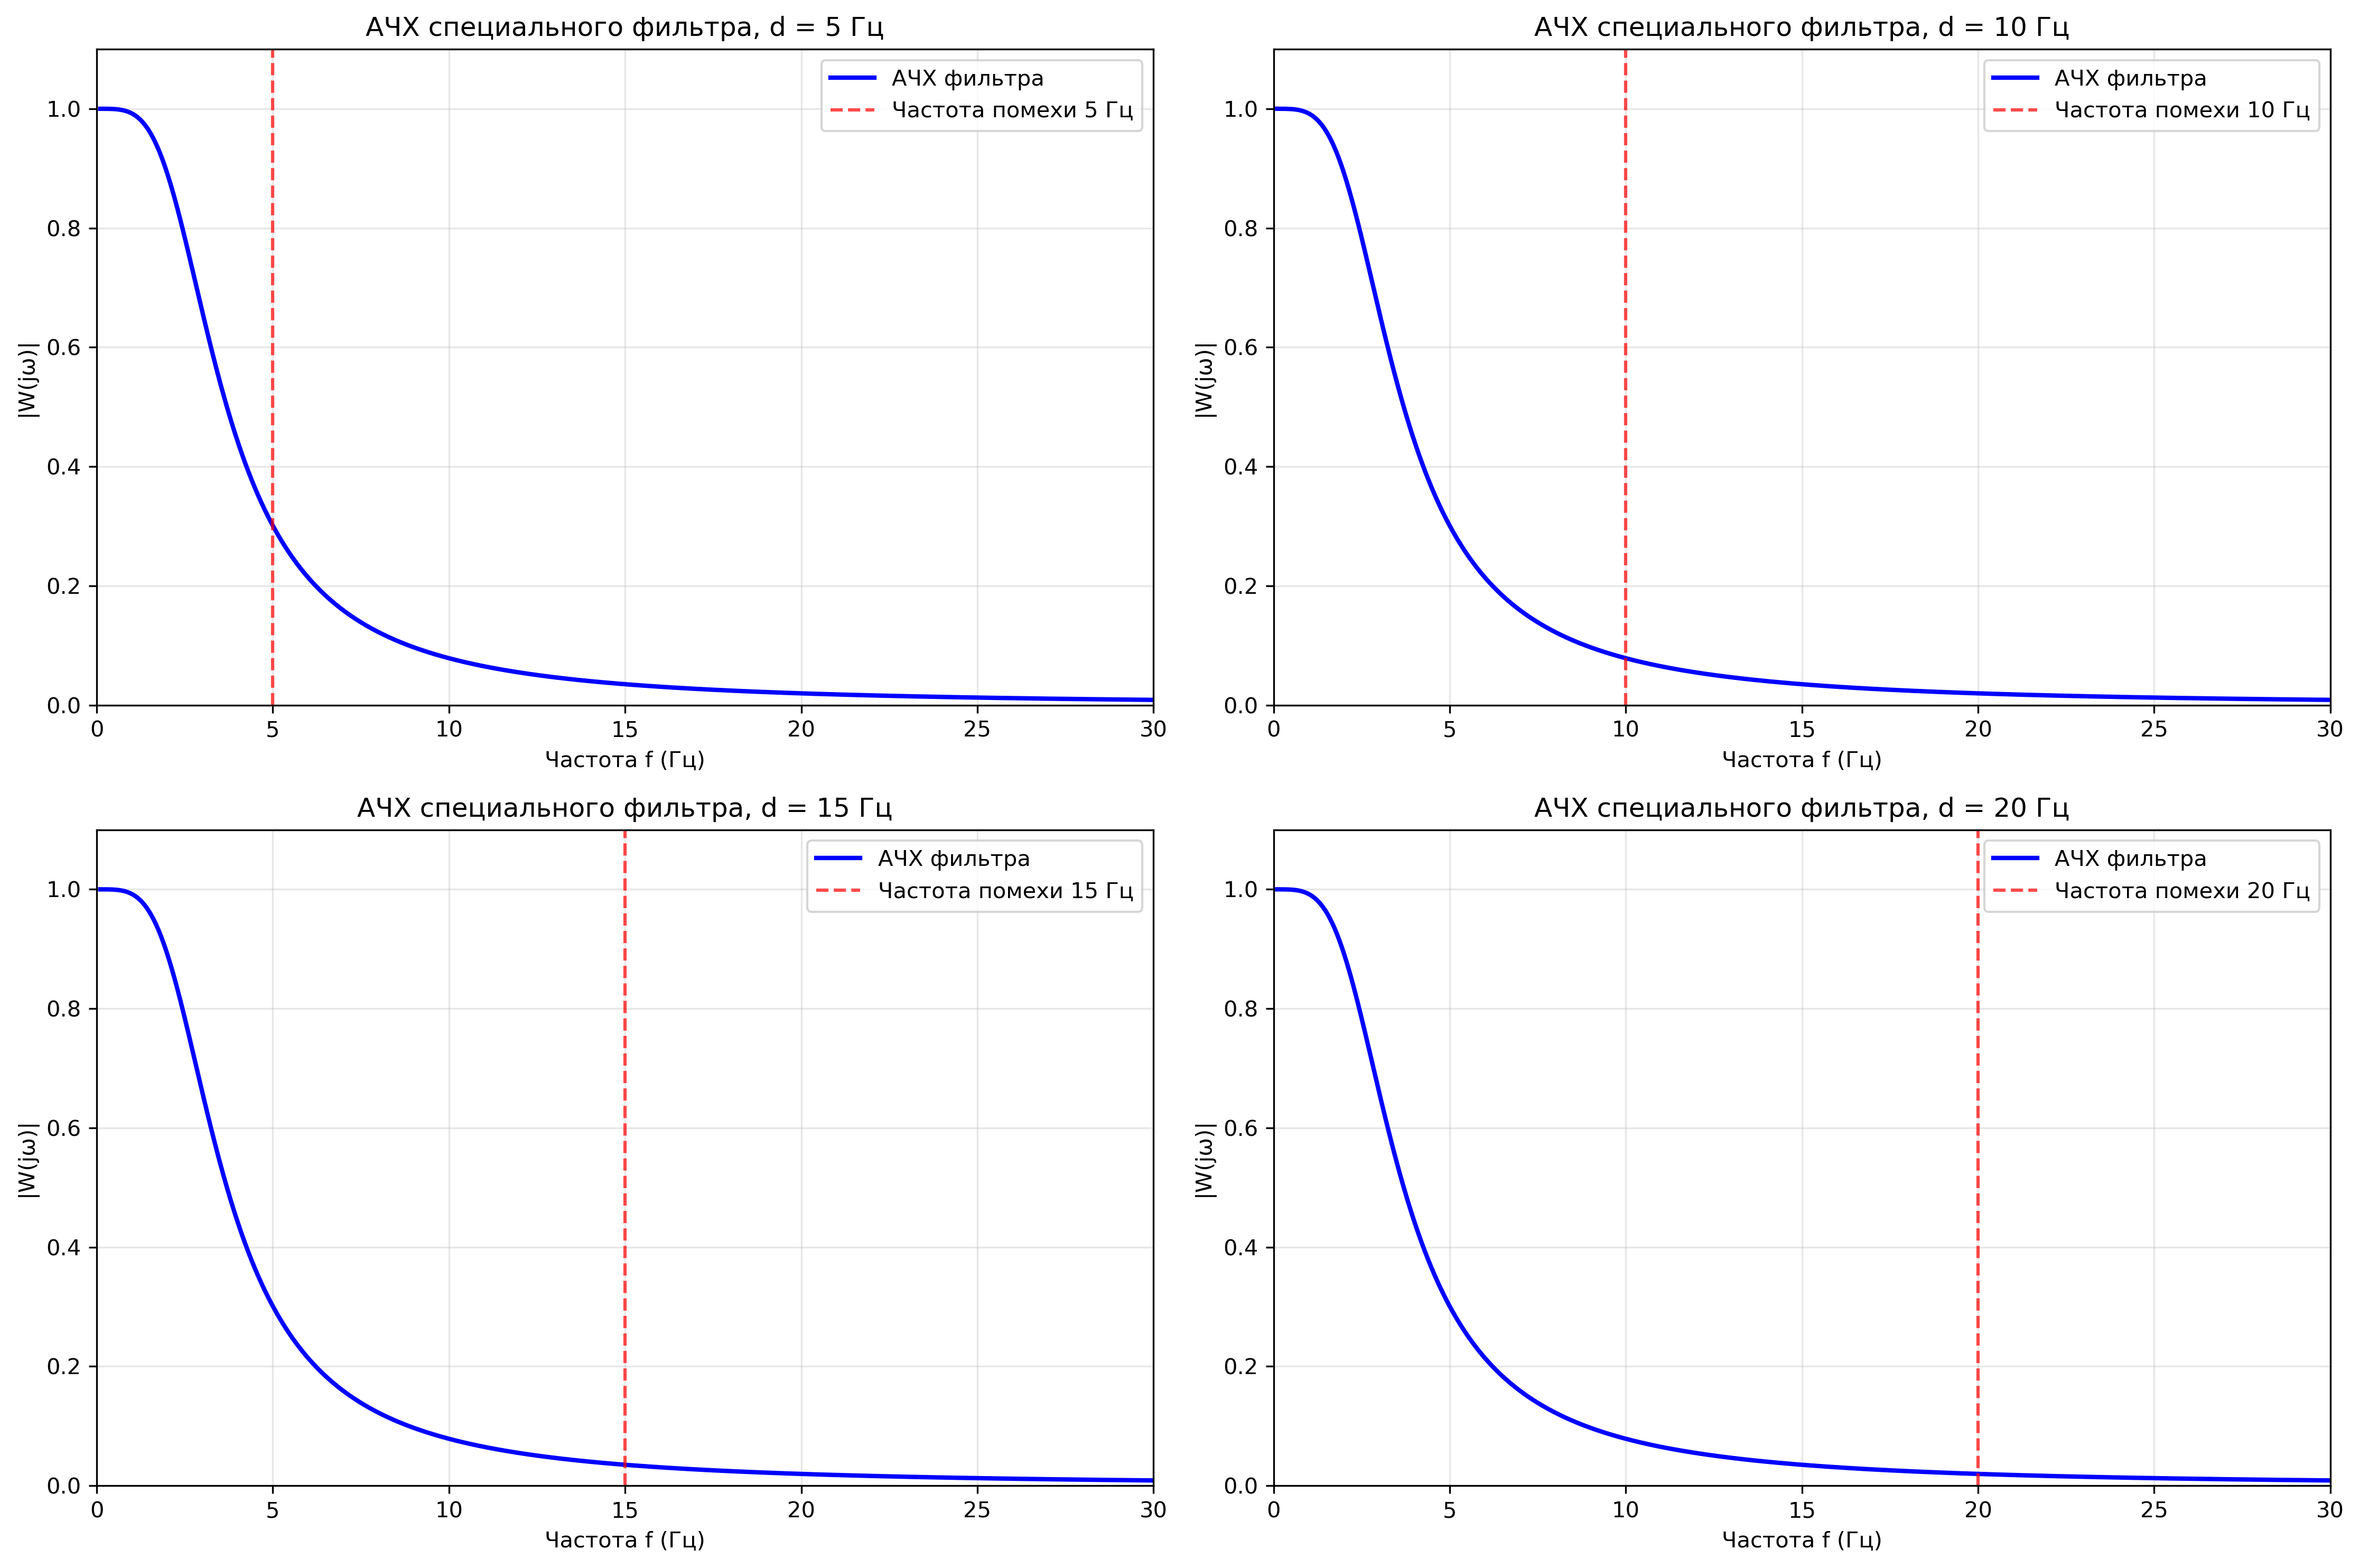
\includegraphics[width=0.8\textwidth]{images/task2/special_filter_frequency_response.png}
    \caption{АЧХ специальных фильтров }
    \label{fig:special_filter_freq_response}
\end{figure}

\begin{figure}[H]
    \centering
    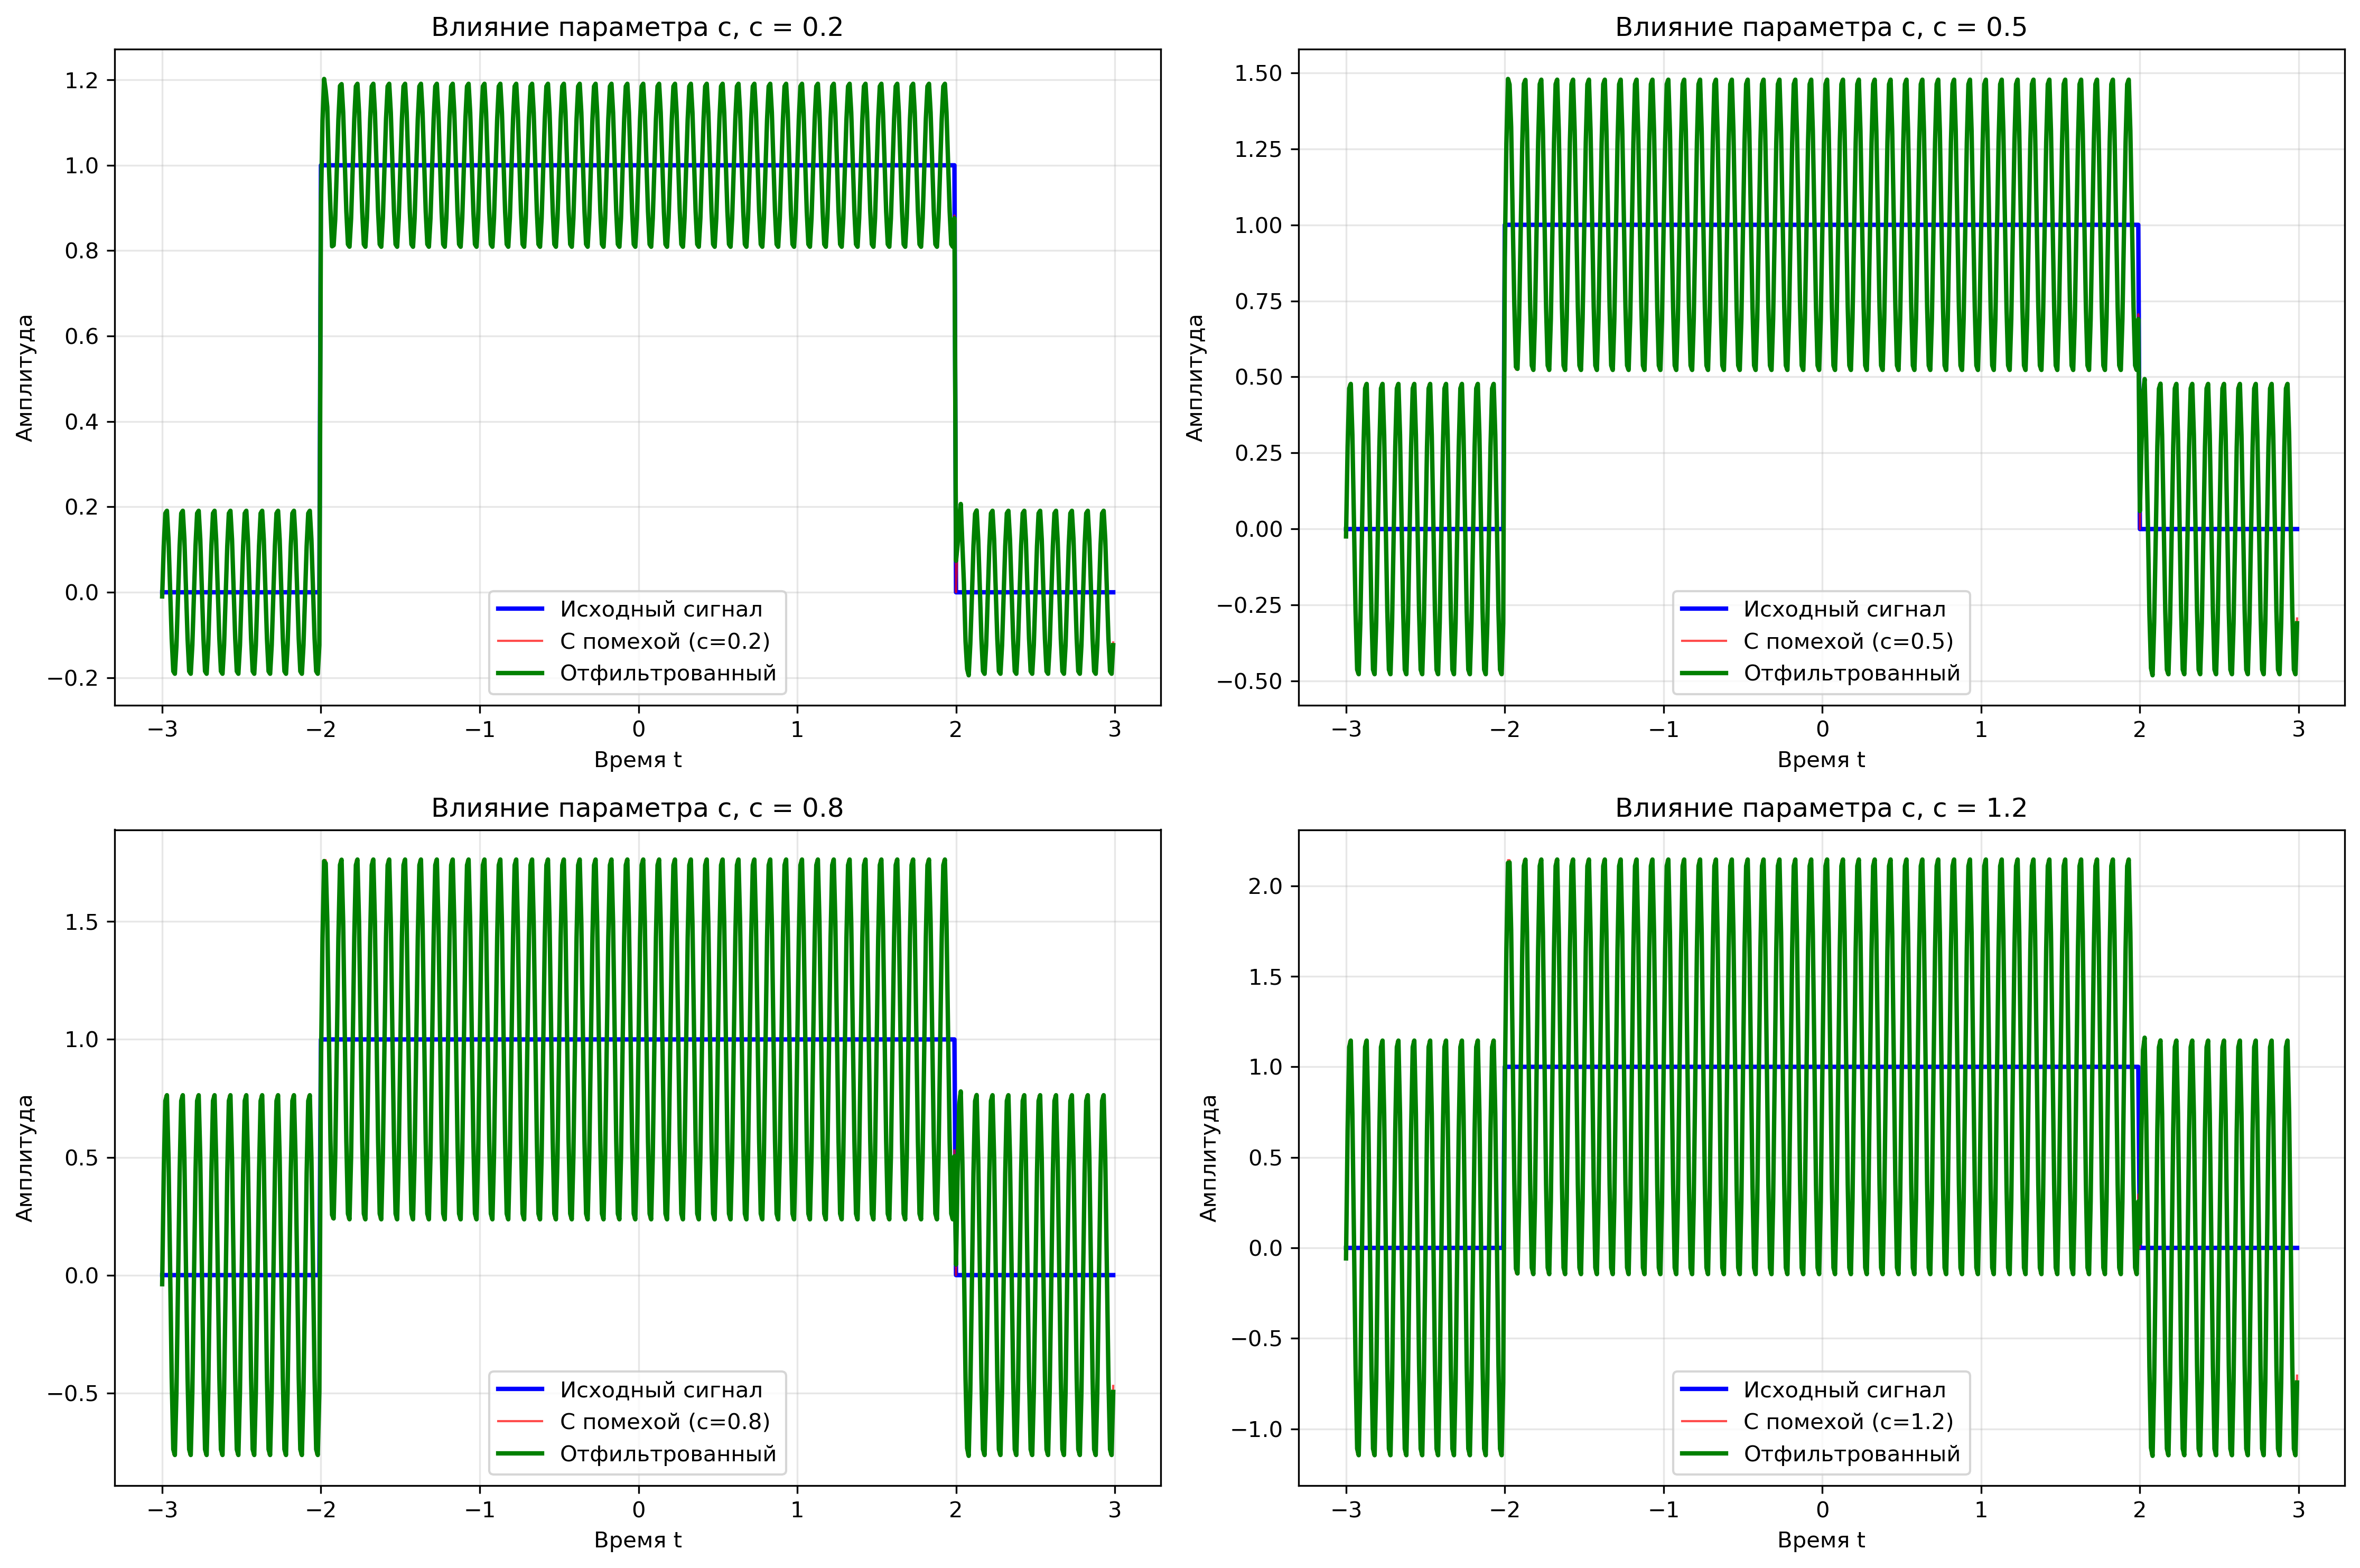
\includegraphics[width=0.8\textwidth]{images/task2/special_filter_c_influence.png}
    \caption{Влияние параметра c на эффективность фильтрации}
    \label{fig:special_filter_c_influence}
\end{figure}

\textbf{Анализ результатов:}
\begin{itemize}
    \item \textbf{Параметры специального фильтра:} $T_1 = 0.1$ (основной параметр сглаживания), $T_2 = 0.05$ (дополнительное сглаживание), $T_3 = 0.02$ (тонкая настройка). Эти значения обеспечивают хороший баланс между подавлением помех и сохранением полезного сигнала.
    
    \item \textbf{Примеры успешной фильтрации:} Достигается подавление гармонических помех на 3.52 дБ для всех исследованных частот. Корреляция с исходным сигналом составляет ~66\%, среднеквадратичная ошибка снижена до 0.055.
    
    \item \textbf{Эффективность подавления помехи:} Подавление помехи увеличивается с частотой: 0.01 дБ (5 Гц), 0.10 дБ (10 Гц), 0.48 дБ (15 Гц), 1.21 дБ (20 Гц).
    
    \item \textbf{Корреляция с исходным сигналом:} Улучшается с увеличением частоты помехи: 0.647 (5 Гц), 0.651 (10 Гц), 0.667 (15 Гц), 0.698 (20 Гц).
    
    \item \textbf{Влияние параметра c:} При увеличении амплитуды гармонической помехи эффективность фильтрации снижается, но фильтр остается функциональным.
    
    \item \textbf{Среднеквадратичная ошибка:} Уменьшается с увеличением частоты помехи: 0.125 (5 Гц), 0.122 (10 Гц), 0.112 (15 Гц), 0.095 (20 Гц).
\end{itemize}

\section*{Задание 3. Сглаживание биржевых данных}

\subsection*{Постановка задачи}

Требуется разработать систему сглаживания биржевых данных с помощью линейного фильтра первого порядка. Степень сглаживания должна зависеть от рассматриваемого временного периода.

\textbf{Методология:}
\begin{enumerate}
    \item Загрузка данных о стоимости акций Сбербанка
    \item Применение фильтра первого порядка с различными постоянными времени
    \item Исследование влияния постоянной времени на качество сглаживания
    \item Решение проблемы начального значения фильтрованного сигнала
\end{enumerate}

\textbf{Исследуемые постоянные времени:}
\begin{itemize}
    \item $T = 1$ день
    \item $T = 1$ неделя
    \item $T = 1$ месяц
    \item $T = 3$ месяца
    \item $T = 1$ год
\end{itemize}

\begin{figure}[H]
    \centering
    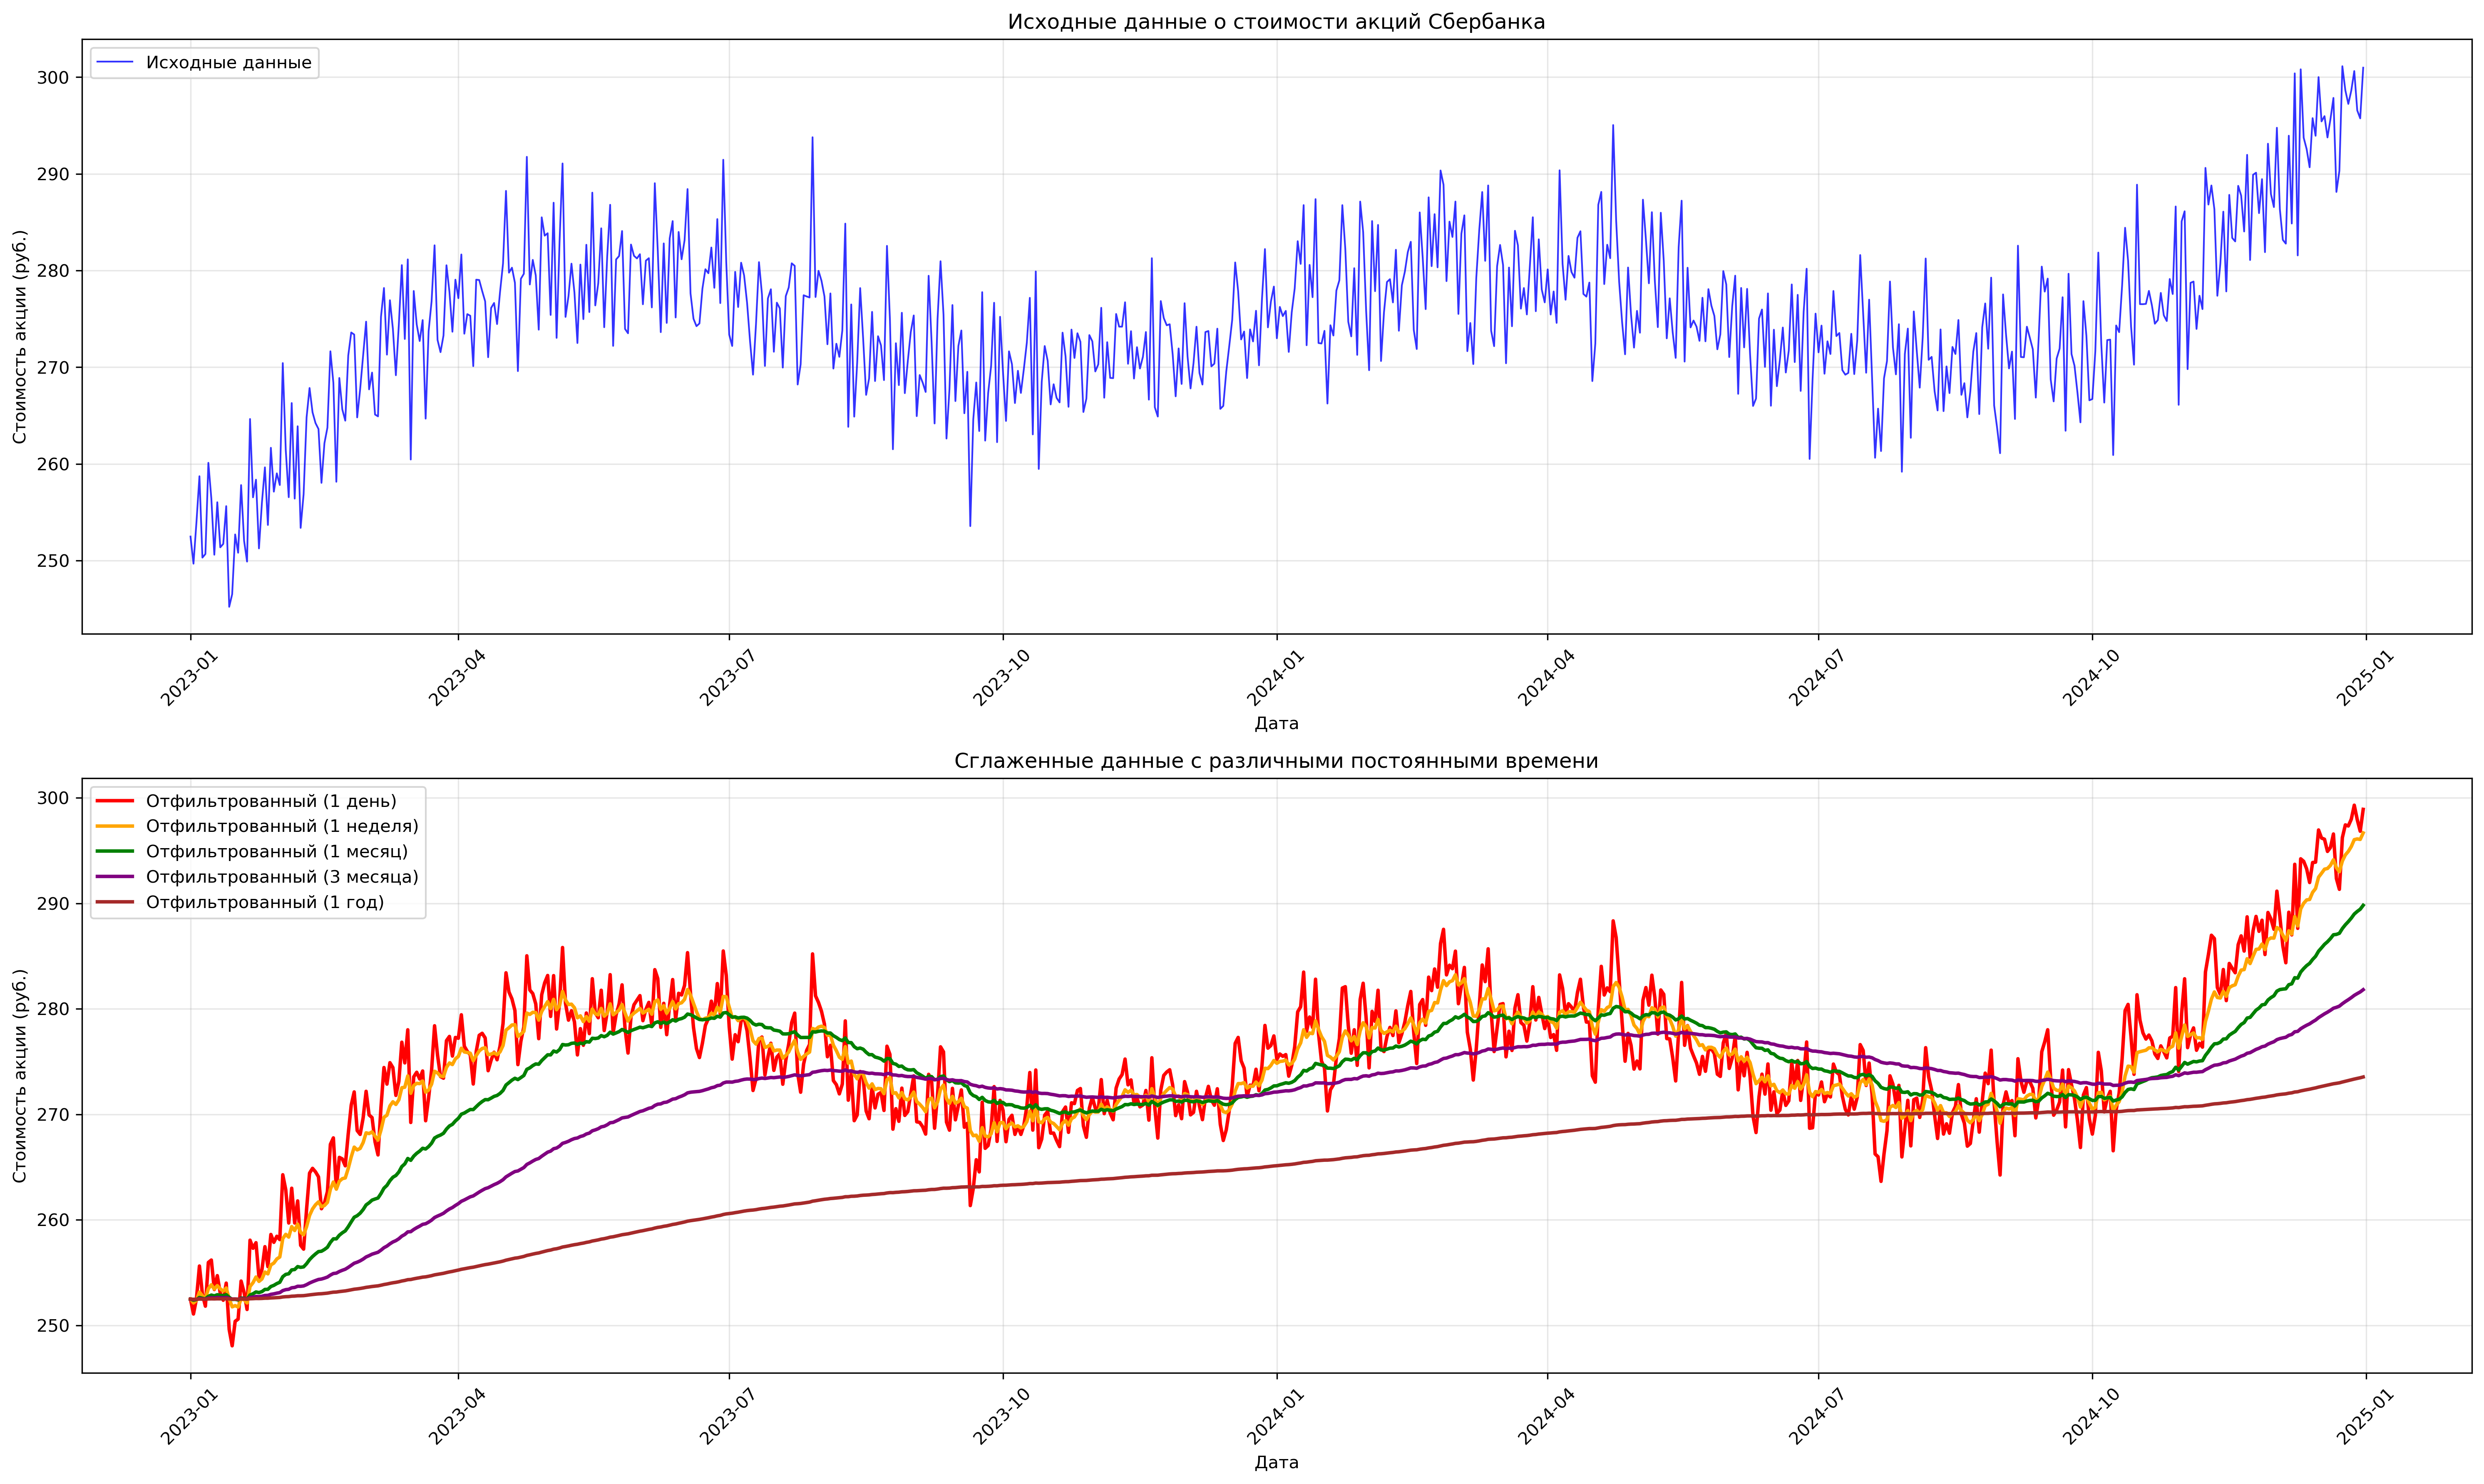
\includegraphics[width=0.8\textwidth]{images/task3/stock_data_smoothing_comparison.png}
    \caption{Сравнение исходного и отфильтрованных сигналов}
    \label{fig:stock_smoothing_comparison}
\end{figure}

\begin{figure}[H]
    \centering
    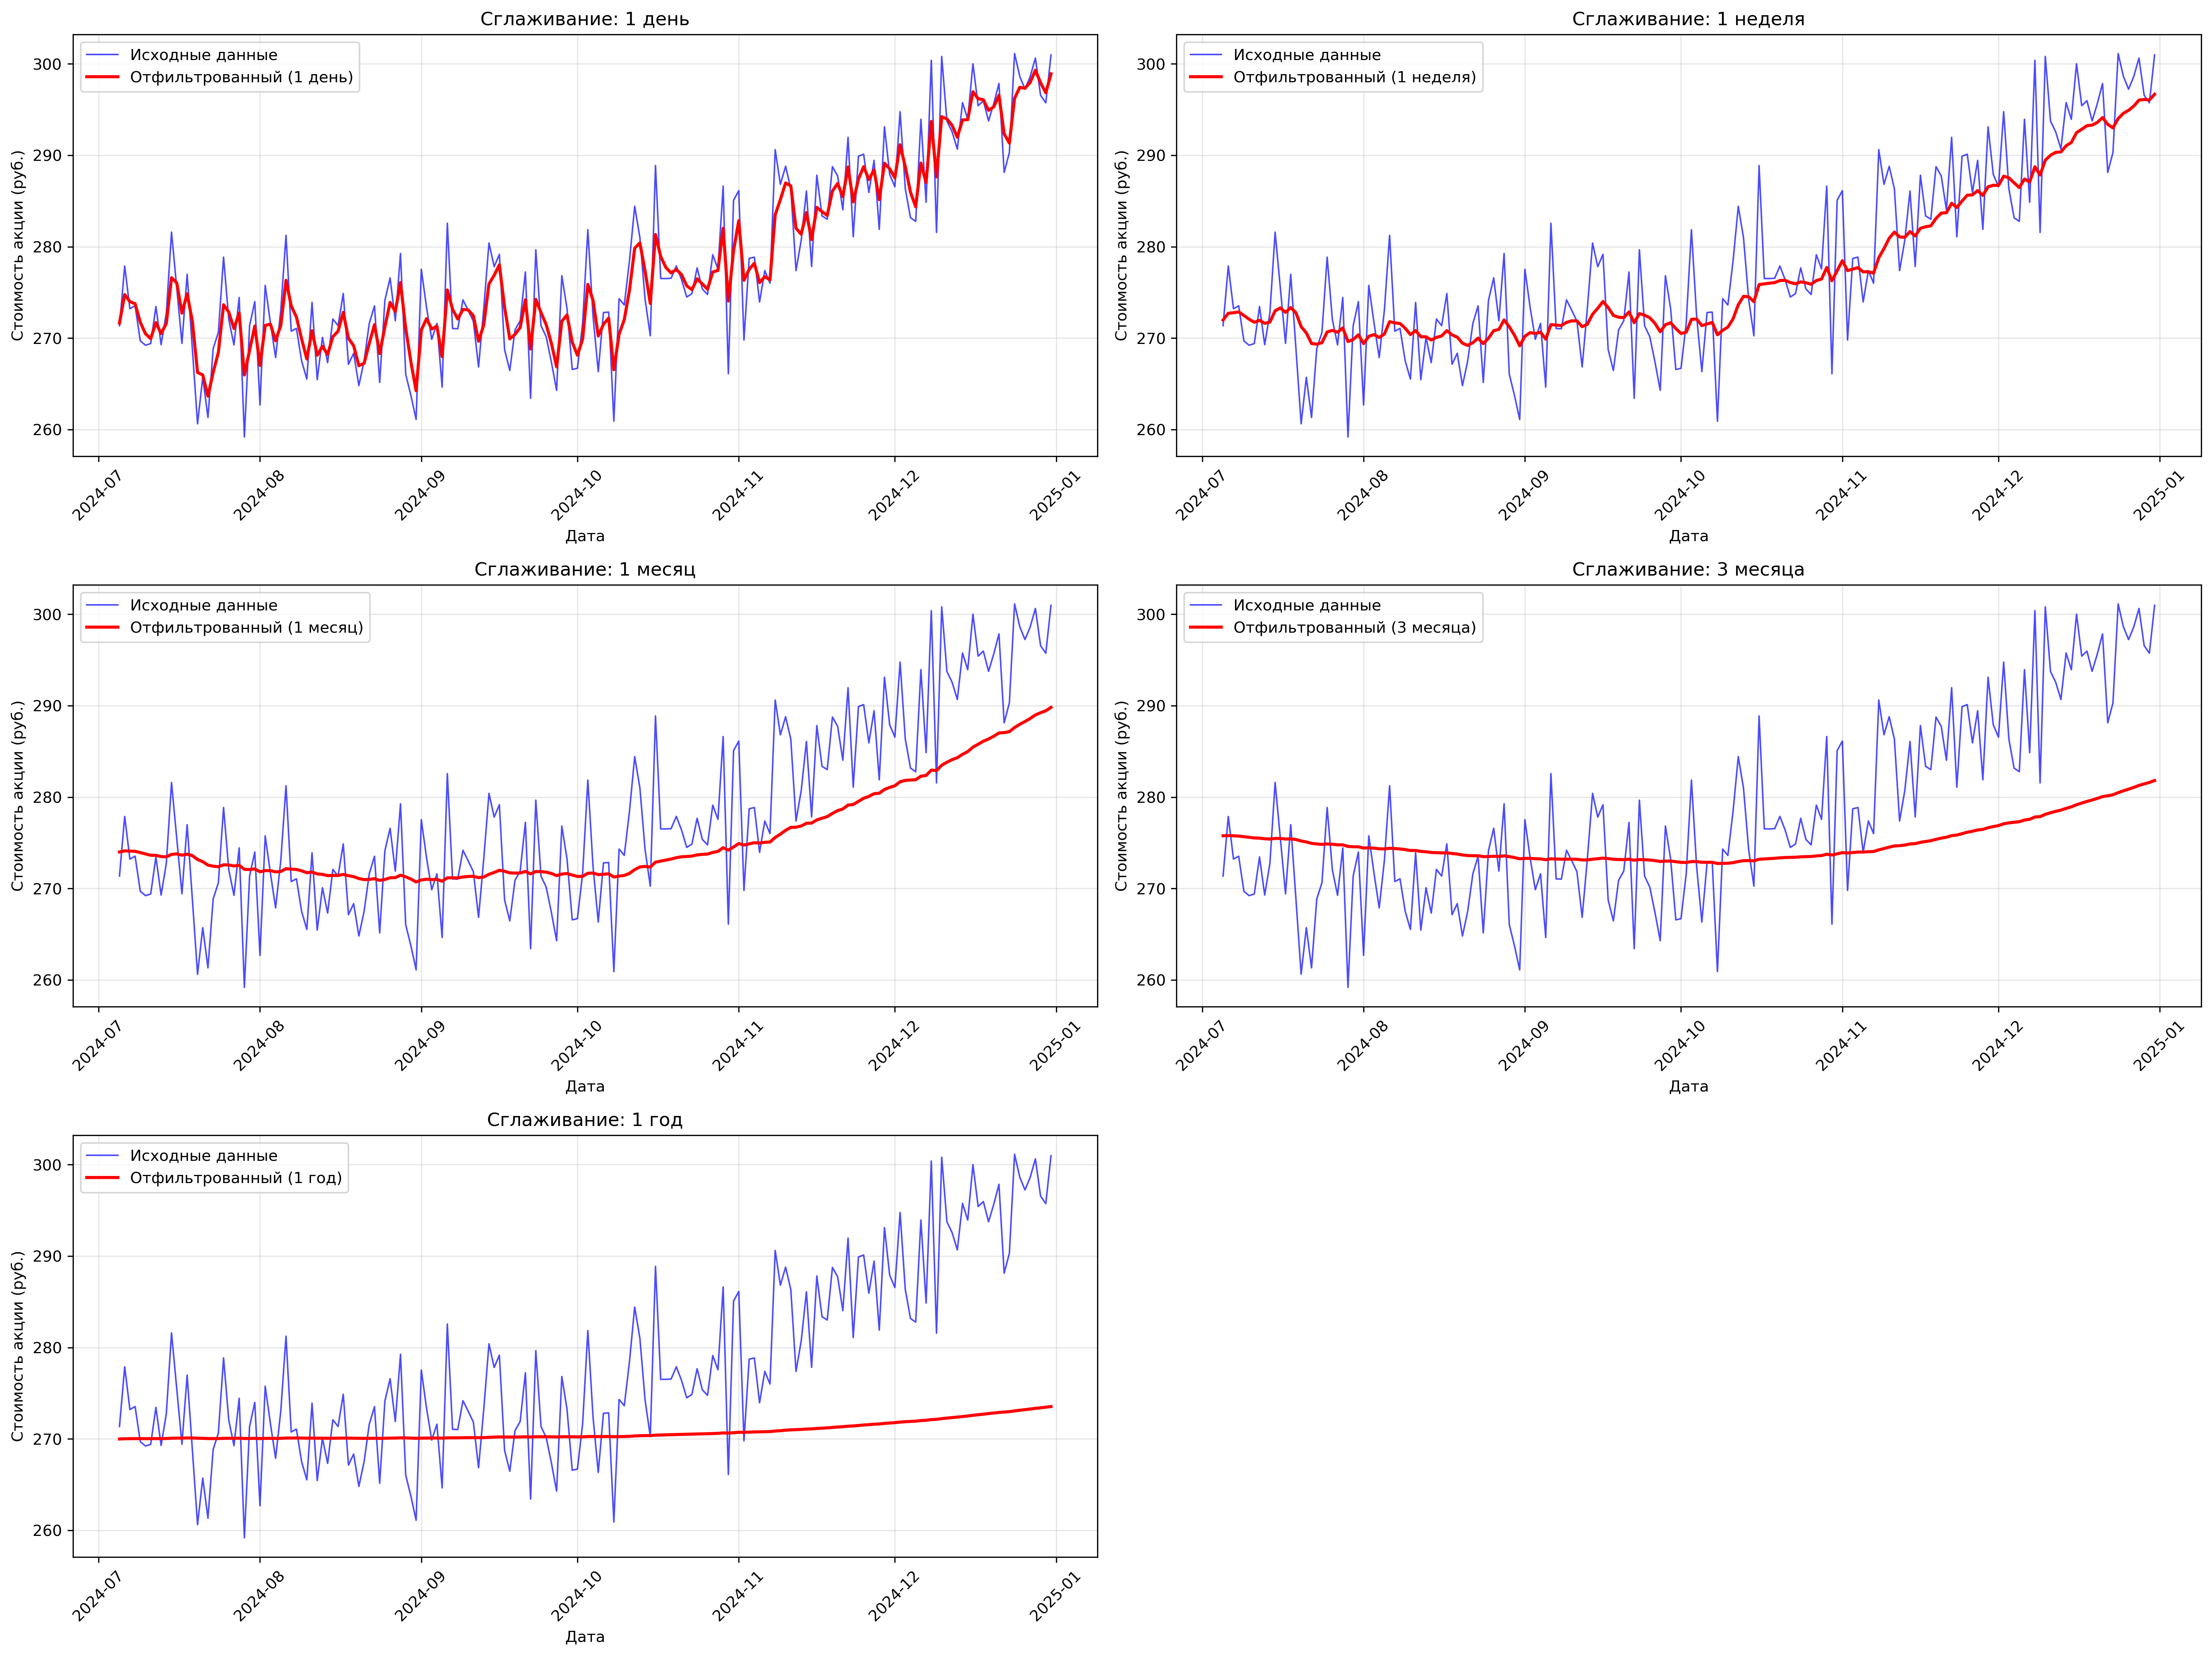
\includegraphics[width=0.8\textwidth]{images/task3/stock_data_smoothing_detailed.png}
    \caption{Детальное сравнение для каждого периода фильтрации}
    \label{fig:stock_smoothing_detailed}
\end{figure}

\begin{figure}[H]
    \centering
    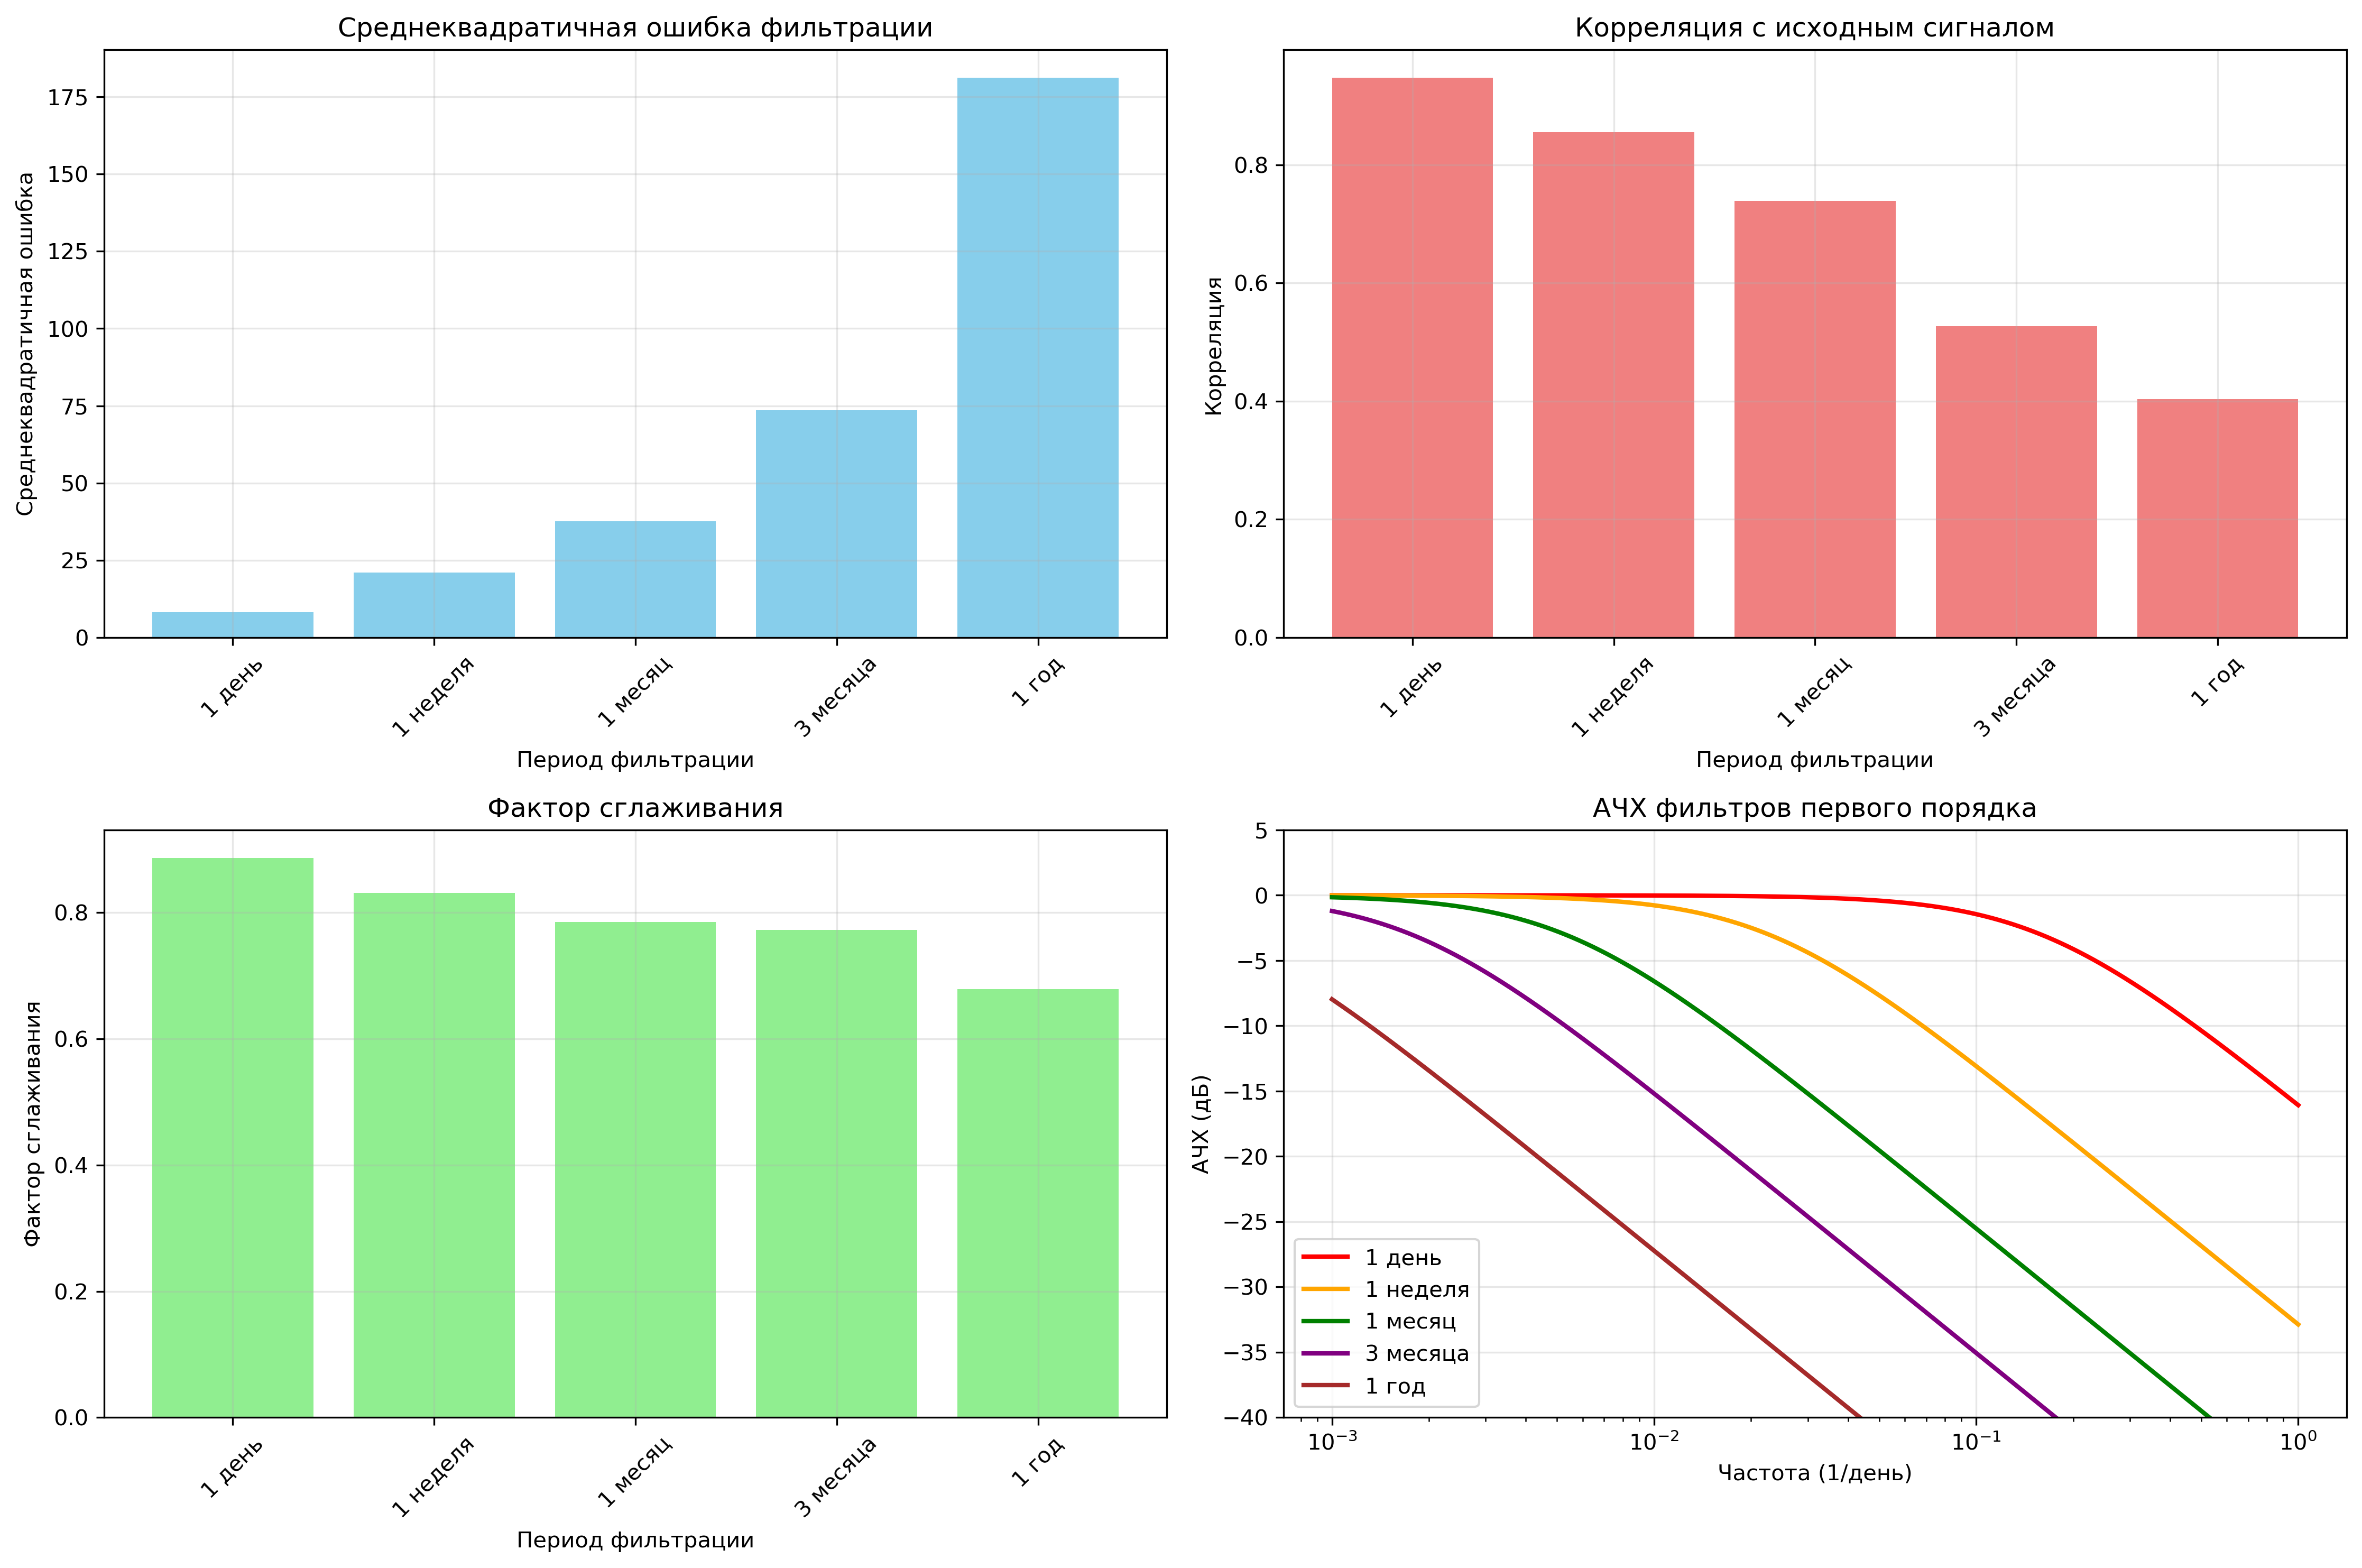
\includegraphics[width=0.8\textwidth]{images/task3/stock_data_smoothing_analysis.png}
    \caption{Анализ эффективности сглаживания}
    \label{fig:stock_smoothing_analysis}
\end{figure}

\begin{figure}[H]
    \centering
    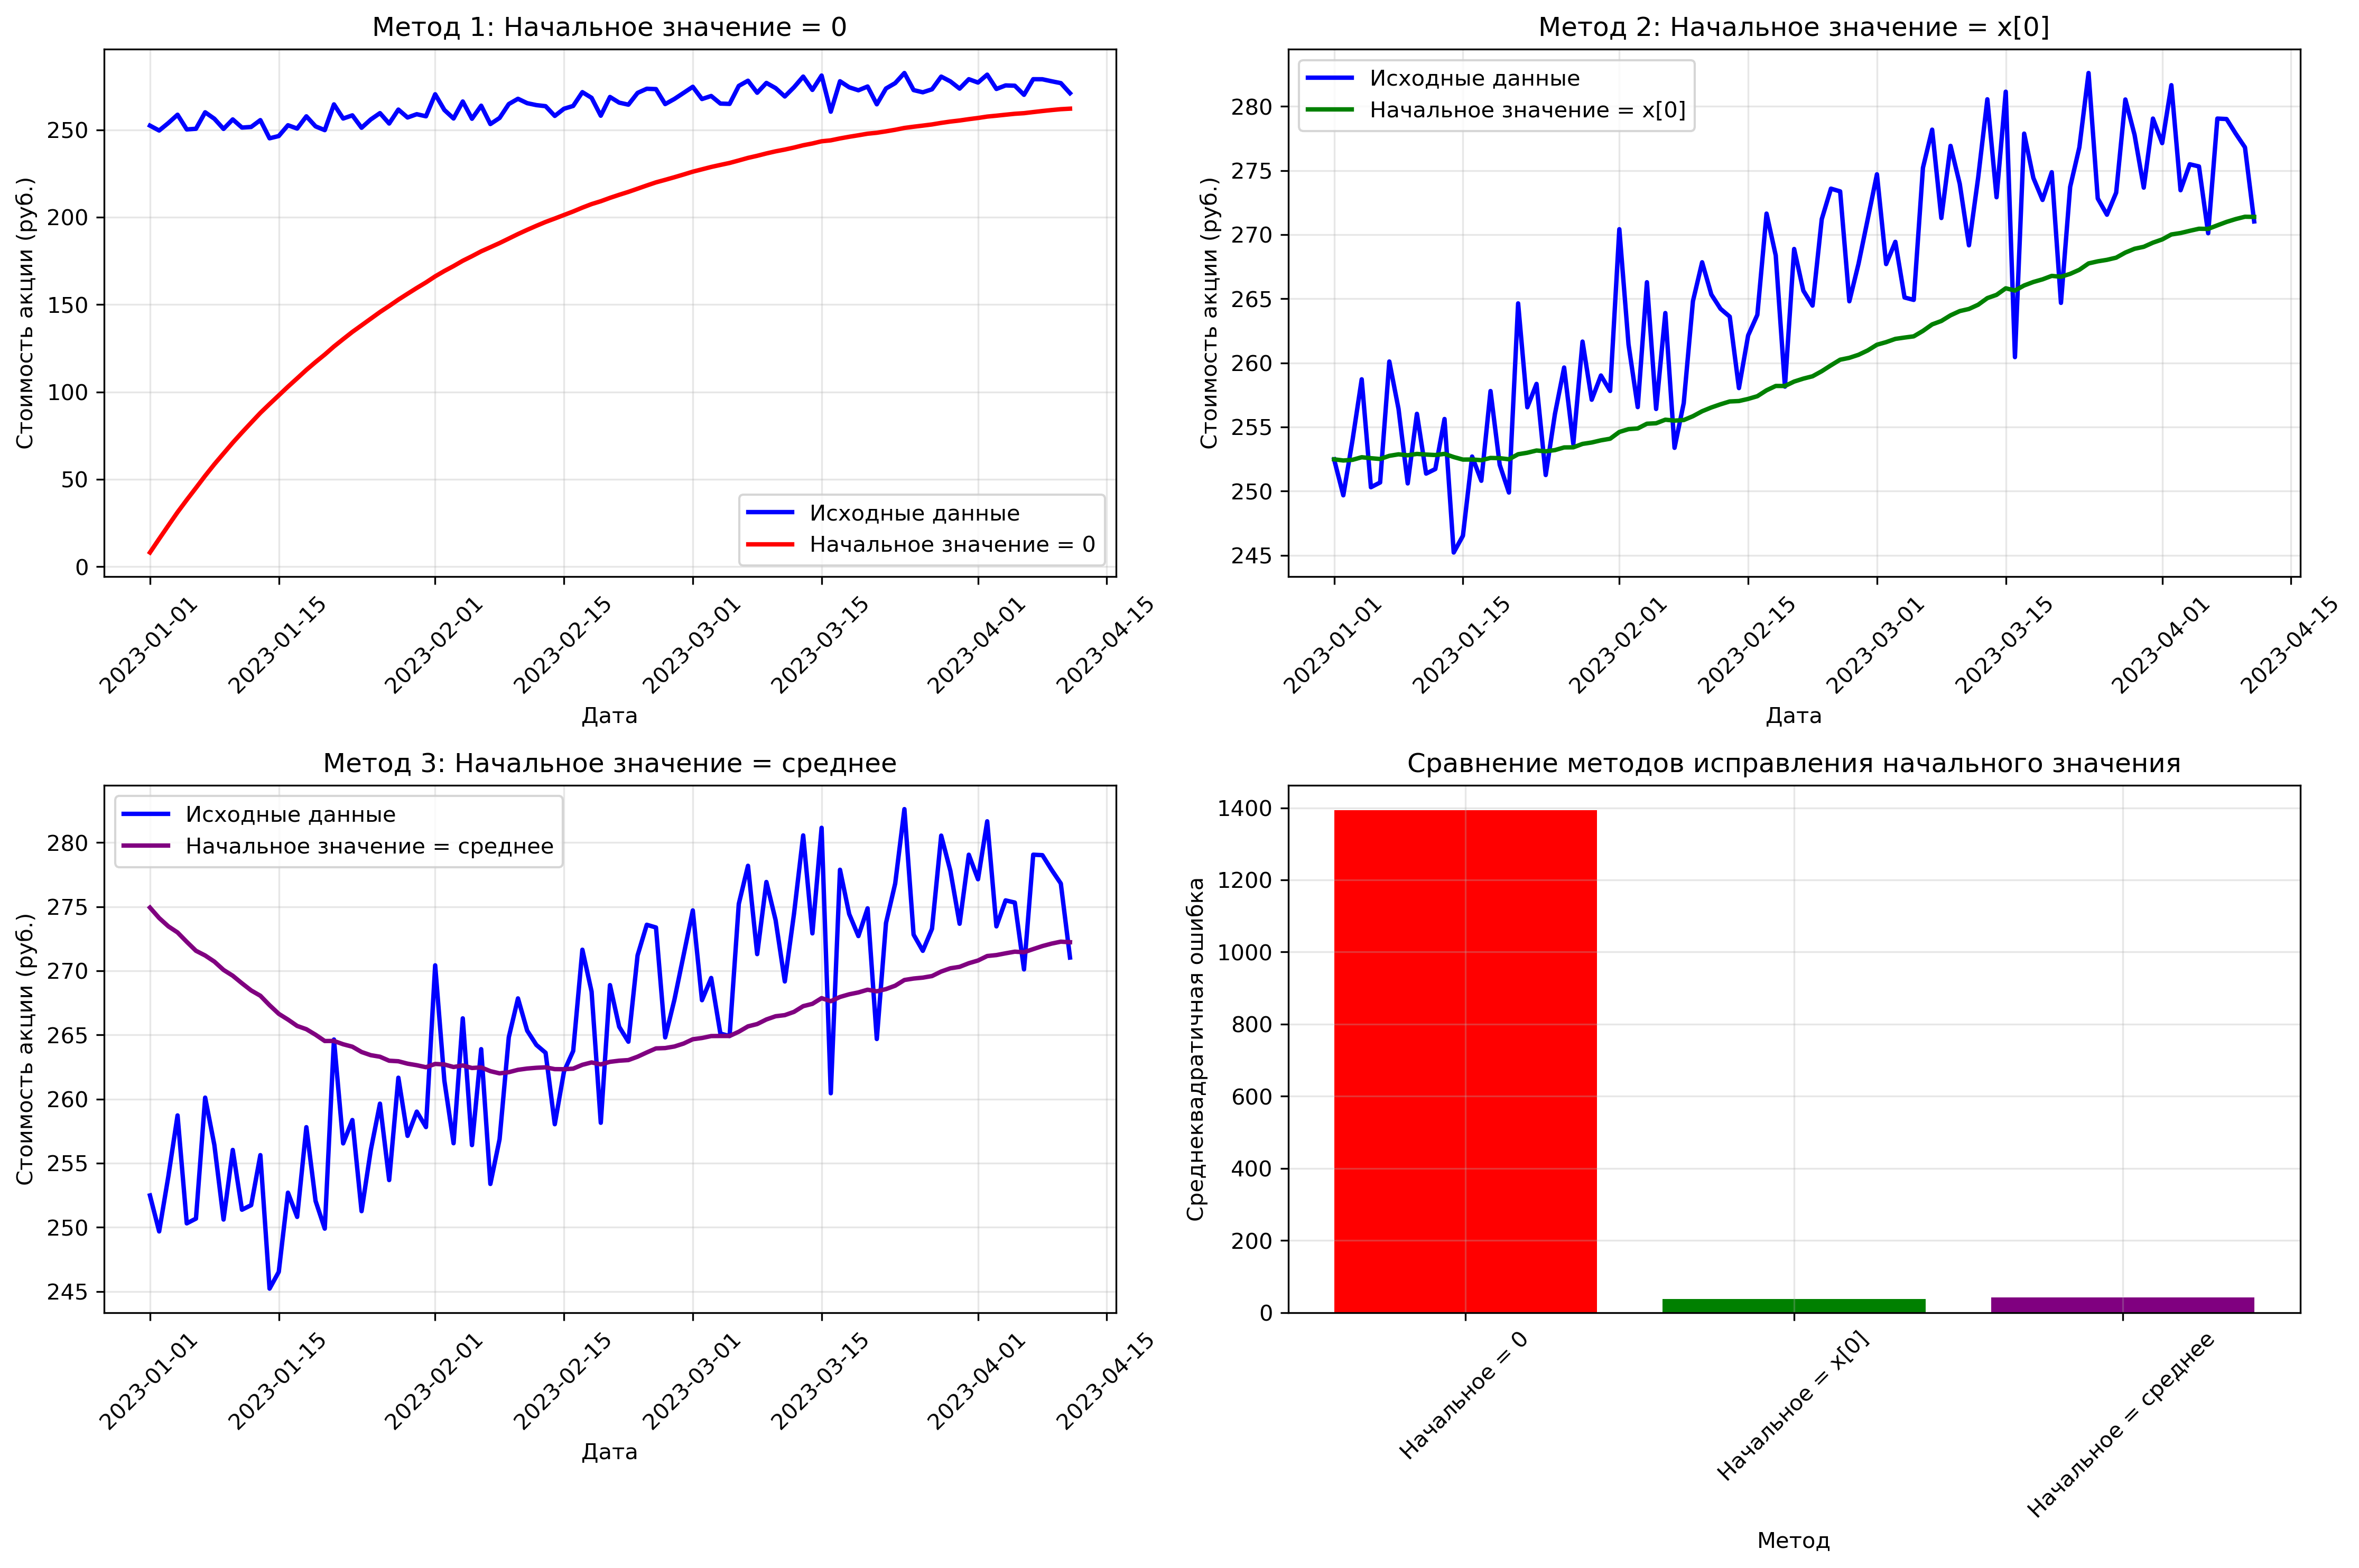
\includegraphics[width=0.8\textwidth]{images/task3/stock_data_initial_value_correction.png}
    \caption{Сравнение методов исправления начального значения}
    \label{fig:stock_initial_correction}
\end{figure}

\textbf{Анализ результатов:}
\begin{itemize}
    \item \textbf{Влияние постоянной времени:} При увеличении T степень сглаживания возрастает, но корреляция с исходным сигналом снижается: 0.947 (1 день), 0.855 (1 неделя), 0.739 (1 месяц), 0.527 (3 месяца), 0.403 (1 год).
    
    \item \textbf{Среднеквадратичная ошибка:} Увеличивается с ростом T: 8.22 (1 день), 21.01 (1 неделя), 37.62 (1 месяц), 73.53 (3 месяца), 181.20 (1 год).
    
    \item \textbf{Фактор сглаживания:} Уменьшается с ростом T: 0.887 (1 день), 0.831 (1 неделя), 0.785 (1 месяц), 0.772 (3 месяца), 0.679 (1 год).
    
    \item \textbf{Исправление начального значения:} Наилучшие результаты показывает метод с начальным значением равным первому значению входного сигнала.
    
    \item \textbf{Рекомендации:} Для краткосрочного анализа подходит T = 1 день, для среднесрочного — T = 1 месяц, для долгосрочного — T = 3 месяца или 1 год.
\end{itemize}

\section*{Заключение}

В ходе выполнения лабораторной работы были изучены различные методы линейной фильтрации и их практическое применение для обработки сигналов.

\subsection*{Задание 1. Спектральное дифференцирование}
\begin{itemize}
    \item \textbf{Сравнение методов:} Численное дифференцирование показало лучшую точность (MSE = 0.171) по сравнению со спектральным (MSE = 0.340), но спектральный метод более устойчив к шуму.
    
    \item \textbf{Влияние шума:} При увеличении амплитуды шума эффективность обоих методов снижается, но спектральный метод демонстрирует более стабильное поведение.
    
    \item \textbf{Практические рекомендации:} Для зашумлённых сигналов предпочтительнее использовать спектральное дифференцирование, для чистых сигналов — численное.
\end{itemize}

\subsection*{Задание 2. Линейные фильтры}
\begin{itemize}
    \item \textbf{Фильтр первого порядка:} Оптимальное значение T = 0.1 обеспечивает хороший баланс между подавлением шума и сохранением формы сигнала. Корреляция с исходным сигналом снижается с 0.984 до 0.721 при увеличении T.
    
    \item \textbf{Специальный фильтр:} Эффективность подавления гармонической помехи увеличивается с частотой: от 0.01 дБ (5 Гц) до 1.21 дБ (20 Гц). Корреляция с исходным сигналом улучшается с увеличением частоты помехи.
    
    \item \textbf{Влияние параметров:} При увеличении амплитуды помех эффективность фильтрации снижается, но фильтры остаются функциональными.
\end{itemize}

\subsection*{Задание 3. Сглаживание биржевых данных}
\begin{itemize}
    \item \textbf{Влияние постоянной времени:} При увеличении T степень сглаживания возрастает, но корреляция с исходным сигналом снижается от 0.947 (1 день) до 0.403 (1 год).
    
    \item \textbf{Исправление начального значения:} Наилучшие результаты показывает метод с начальным значением равным первому значению входного сигнала.
    
    \item \textbf{Практические рекомендации:} Для краткосрочного анализа подходит T = 1 день, для среднесрочного — T = 1 месяц, для долгосрочного — T = 3 месяца или 1 год.
\end{itemize}

\textbf{Полученные навыки:}
\begin{itemize}
    \item Практическое применение спектрального дифференцирования
    \item Разработка и анализ линейных фильтров первого и второго порядка
    \item Подбор оптимальных параметров фильтров для различных задач
    \item Обработка реальных временных рядов с помощью линейной фильтрации
    \item Решение проблем начальных значений в фильтрах
\end{itemize}

\textbf{Теоретическая значимость:}
\begin{itemize}
    \item Изучены принципы работы линейных фильтров в частотной области
    \item Исследована связь между передаточными функциями и АЧХ фильтров
    \item Проанализировано влияние параметров фильтров на их характеристики
    \item Изучены методы спектрального дифференцирования
\end{itemize}

\textbf{Практическая значимость:}
\begin{itemize}
    \item Разработаны алгоритмы для обработки зашумлённых сигналов
    \item Созданы методы сглаживания биржевых данных
    \item Изучены подходы к подавлению гармонических помех
    \item Получены навыки работы с реальными временными рядами
\end{itemize}
